\documentclass[12pt, a4paper]{article}
% pacotes utilizados
%\usepackage{abnt-UFPR}
\usepackage[pdftex]{graphicx}
\usepackage{graphicx,url}
\usepackage[utf8]{inputenc}
\usepackage[brazil]{babel}
\usepackage{setspace}
\onehalfspace
\usepackage{enumerate}
\usepackage{multirow}
\usepackage{parskip}
\usepackage{float}
\usepackage{color}
\usepackage[normalem]{ulem}
\usepackage{lmodern}
\usepackage{pdfpages}

\usepackage{listings}

\definecolor{verdao}{rgb}{0.0, 0.5, 0.0}

\lstset{
	language=Python,
	frame=single,
	numbers=left,
	showspaces=false,
	showstringspaces=false,
	basicstyle=\ttfamily,
	captionpos=t,
	basicstyle=\small,
	keywordstyle=\ttfamily \color{blue},
	keywordstyle=[2]\ttfamily \color{blue},
	stringstyle=\color{red}\ttfamily,
	commentstyle=\color{verdao}\ttfamily
}

%\usepackage{fancyhdr}
\usepackage{indentfirst}
\usepackage[a4paper,left=3cm,right=2cm,top=3cm,bottom=2cm]{geometry}
\usepackage[alf]{abntex2cite}
%\pagestyle{headings}
%configuracoes do sumario
\usepackage{tocloft}
\renewcommand{\cftdot}{\textbf{.}}
\renewcommand{\cftsecdotsep}{\cftdotsep}
\renewcommand{\cftsecdotsep}{4}
\renewcommand{\cftsubsecdotsep}{4}
\renewcommand{\cftsecfont}{\normalsize\bfseries}
\renewcommand{\cftsubsecfont}{\normalsize}
\renewcommand{\cftsecpagefont}{\textbf}
\renewcommand{\cftsubsecpagefont}{\textbf}
\cftsetindents{section}{0cm}{1.3cm}
\cftsetindents{subsection}{0cm}{1.3cm}
\cftsetindents{subsubsection}{0cm}{1.3cm}
%\renewcommand{\figurename}{Fig.}
\newcommand{\bigsize}{\fontsize{12pt}{20pt}\selectfont}

\usepackage[labelsep=endash]{caption}
\setlength{\cftsubsecindent}{0em}
\tocloftpagestyle{empty}
\newcommand{\bfemph}[1]{\textbf{\textit{#1}}}
\renewcommand{\emph}[1]{\bfemph{#1}}
%Formatacao de Padroes das Referencias Bibliograficas
%\usepackage{custom-bib}

%Formatacao de Titulos, Secoes, Subtitulos, etc...
\usepackage{titlesec}
\titleformat{\section}{\normalfont\normalsize\filright\bfseries}{\thesection}{1em}{\uppercase}
%\renewcommand{\thesubsection}{\alph{subsection}}
\titleformat{\subsection}{\normalfont\normalsize\filright\bfseries}{\thesubsection}{1em}{}
%\renewcommand{\thesubsubsection}{\roman{subsubsection}}
\titleformat{\subsubsection}{\normalfont\normalsize\bfseries}{\thesubsubsection}{1em}{}
%

%Espacamento de Paragrafos
\setlength{\parindent}{0.8cm}
\setlength{\parskip}{1ex plus 0.5ex minus 0.2ex}
%1ex plus 0.5ex minus 0.2ex
\pagestyle{myheadings}

\pagenumbering{arabic}

\author{ \bf UNIVERSIDADE DO ESTADO DO AMAZONAS - UEA \\[14pt] \small ESCOLA SUPERIOR DE TECNOLOGIA - EST \\[14pt] ENGENHARIA ELÉTRICA \\[96pt] CARLA PATRICIA MICHILES ARAUJO \\[96pt]}
\title{ \rm \bf \Large SISTEMA DE AQUISIÇÃO DE SINAIS ELETROCARDIOGRÁFICOS UTILIZANDO TECNOLOGIA WIRELESS\\[123pt] \rm \small Manaus \\  2018}




\pagestyle{myheadings}

% Start the document
\begin{document}

\addtocontents{toc}{\protect\thispagestyle{empty}}
%INÍCIO DA CAPA DA MONOGRAFIA
\thispagestyle{empty}
\begin{center}
\textbf{ UNIVERSIDADE DO ESTADO DO AMAZONAS \\
ESCOLA SUPERIOR DE TECNOLOGIA \\[50pt] }
\textbf{ \\[70pt] {\bigsize CARLA PATRICIA MICHILES ARAUJO} \\[120pt] }
\textbf{ {\bigsize SISTEMA DE AQUISIÇÃO DE SINAIS ELETROCARDIOGRÁFICOS UTILIZANDO TECNOLOGIA WIRELESS}  \\[104pt] }
\end{center}
% COMENTÁRIOS DA FOLHA DE ROSTO
\hspace*{8cm}

\vspace*{\fill}

\begin{center}
Manaus \\ 2017
\end{center}

%FIM DA CAPA DA MONOGRAFIA

%INÍCIO DA FOLHA DE ROSTO
\newpage
\thispagestyle{empty}
\begin{center}


% \textbf{ \\[70pt] {\bigsize CARLA PATRICIA MICHILES ARAUJO} \\[120pt] }
\textbf{ {\bigsize CARLA PATRICIA MICHILES ARAUJO} \\[120pt] }
\textbf{ {\bigsize SISTEMA DE AQUISIÇÃO DE SINAIS ELETROCARDIOGRÁFICOS UTILIZANDO TECNOLOGIA WIRELESS}  \\[50pt] }
\end{center}
% COMENTÁRIOS DA FOLHA DE ROSTO
\hspace*{8cm}
\begin{flushright}
\begin{minipage}{8cm}
\begin{singlespace}
Projeto de pesquisa desenvolvido durante a disciplina de Trabalho de Conclusão de Curso II e apresentada à banca avaliadora do Curso de Engenharia Elétrica da Escola Superior de Tecnologia da Universidade do Estado do Amazonas, como pré-requisito para obtenção do título de Engenheiro Eletricista.\\[50pt]
\end{singlespace}
\end{minipage}
\end{flushright}
\begin{center}
Orientador: Wheidima Carneiro de Melo, Me.

\end{center}

\vspace*{\fill}
\begin{center}
Manaus \\ 2017
\end{center}



%FIM DA FOLHA DE ROSTO

%INICIO DA PAG CATALOGAÇÃO

\newpage
\thispagestyle{empty}

%\begin{figure}[!htb]
%\begin{center}
%			\includegraphics[width=\textwidth]{catt.PNG}
%            \vspace*{\fill} 
%            \begin{quote} 
%            \centering  
%            \end{quote}
%            \vspace*{\fill}
%			\label{fig:cat.PNG}
%\end{center}
%\end{figure}


\includepdf[pages=-]{carlaze.pdf}

\newpage
\thispagestyle{empty}
\begin{center}


% \textbf{ \\[30pt] {\bigsize CARLA PATRICIA MICHILES ARAUJO} \\[50pt] }
\textbf{ {\bigsize CARLA PATRICIA MICHILES ARAUJO} \\[50pt] }
\textbf{ {\bigsize SISTEMA DE AQUISIÇÃO DE SINAIS ELETROCARDIOGRÁFICOS UTILIZANDO TECNOLOGIA WIRELESS}  \\[50pt] }
\end{center}
% COMENTÁRIOS DA FOLHA DE ROSTO
\hspace*{8cm}
\begin{flushright}
\begin{minipage}{8cm}
\begin{singlespace}
Pesquisa desenvolvida durante a disciplina de Trabalho de Conclusão de Curso II e apresentada à banca avaliadora do Curso de Engenharia Elétrica da Escola Superior de Tecnologia da Universidade do Estado do Amazonas, como pré-requisito para obtenção do título de Engenharia Eletricista.\\[30pt]
\end{singlespace}
\end{minipage}
\end{flushright}
\begin{center}
Nota obtida:\uline{\hspace{1cm}}(\uline{\hspace{8cm}})
\newline \\
Aprovada em 22/11/2017
\newline\\
Área de concentração: Engenharia Biomédica \,\,\,\,\,\,\,\,\,\,\,\,\,\,\,\,\,\,\,
\end{center}
\vspace{1.2cm}
\begin{center}
BANCA EXAMINADORA
\end{center}
\vspace{1.0cm}

%\begin{flushright}
\begin{minipage}[l]{14cm}
\begin{center}
\hspace{1cm}\uline{\hspace{10.5cm}} \\
\hspace{1cm}Orientador: Wheidima Carneiro de Melo, Me.

\hspace{1cm}\uline{\hspace{10.5cm}} \\
\hspace{1cm}Avaliador: Jozias Parente de Oliveira, Dr.

\hspace{1cm}\uline{\hspace{10.5cm}} \\
\hspace{1cm}Avaliador: Charles Luiz de Melo, Me.

\end{center}
\end{minipage}

%\end{flushright}
\hspace*{8cm}

\vspace*{\fill}
\begin{center}
Manaus\\2017
\end{center}



\newpage
\thispagestyle{empty}
\begin{flushright}
\begin{minipage}{8cm}
\begin{singlespace}
{\begin{center}\vspace{18cm}\textbf{\normalsize Dedicatória}\vspace{36pt}\end{center}}
Dedico este trabalho ao meu irmão Pablo (in memorian) que está presente a toda hora no meu coração e aos momentos de alegria que me proporcionou na sua caminhada.\\[50pt]
\end{singlespace}
\end{minipage}
\end{flushright}
\newpage
\thispagestyle{empty}
\vspace*{4.5cm}
{\begin{center}\textbf{\normalsize AGRADECIMENTO}\vspace{36pt}\end{center}}
\hspace*{0.8cm}À Deus, que tornou possível, mesmo com muitos sacrifícios me deu fé para finalização deste trabalho.

\hspace*{0.8cm} Agradeço á minha família, que sempre proporcionaram condições adequadas para crescer na vida pessoal e profissional e ao meu noivo, amigo e compaheiro de todas as horas, Kenny Vinente, pelo carinho, paciência, compreensão e amor.

\hspace*{0.8cm} Agradeço ao meu orientador, Wheidima Carneiro de Melo, por fornecer todo o apoio que eu precisava para a realização deste trabalho.


\hspace*{0.8cm}Aos engenheiros, Thales Araujo, Ronald Santos e Adriano Ibrahim, pelo tempo dedicado na empresa Philips, que contribuiram com material e suporte no entendimento teórico do sinal do eletrocardiograma.


\hspace*{0.8cm}Aos alunos de graduação, Giovanni Antonnacio e Marcus Vinícius pelo suporte no desenvolvimento do projeto e aos Notáveis que estiveram ao meu lado me incentivando durante todo o processo.




\newpage


\thispagestyle{empty}
\vspace*{4.4cm}
{\begin{center}\textbf{\normalsize RESUMO}\vspace{36pt}\end{center}}
\textcolor{red}{Mude isso! No resumo vc dará uma visão geral do trabalho. Então é como se vc colocasse um pouquinho da intro, desen e conclu...sacou?}
O presente trabalho tem como objetivo desenvolver um protótipo de eletrocardiógrafo portátil de baixo custo que realize a aquisição e transmissão dos sinais ECG em tempo real. Sua apresentação está dividida em quatro capítulos. O primeiro capítulo, Referencial Teórico, apresenta assuntos referente a composição do eletrocardiograma, necessárias para o desenvolvimento deste trabalho, o coração, o ciclo cardíaco, o eletrocardiograma, derivações eletrocardiográficas, o triângulo de einthoven, eletrodos e interferência em sinais de ECG. O segundo capítulo, Metodologia, apresenta os materias e métodos necessário para aquisição e transmissão dos sinais de ECG. O terceiro capítulo, Implementação do Projeto, descreve o uso dos componentes, assim como o desenvolvimento do hardware utilizando a placa de aquisição e o Rapsberry Pi 3, além de descrever o uso dos protocolos utilizados, o funcionamento da arquitetura cliente-servidor para transmissão de dados utilizando a rede Wi-Fi como meio de comunicação. O quarto capítulo apresenta os resultados obtidos durante o desenvolvimento do projeto. Apesar do estudo ter um caráter de implementação do circuito de aquisição ECG, os resultados obtidos apresentaram ruídos nas formas de ondas, que poderiam ser diminuídos se algoritmos específicos com certo grau de complexidade fossem utilizados para realizar a separação do sinal e ruído. Nas conclusões são apresentadas as dificuldades enfrentadas na realização deste projeto, os objetivos que foram alcançados e aplicações para o protótipo desenvolvido.


\textbf{Palavras chave}: eletrocardiograma. protótipo de baixo custo, Raspberry Pi 3 \textcolor{red}{Mude tbm! Aqui tem q ser algo que esteja diretamente ligado ao seu trabalho. SUGESTÃO: SISTEMA DE AQUISIÇÃO DE ECG, DISPOSITIVO PORTÁTIL, ENGENHARIA BIOMÉDICA}.  
\newpage
\thispagestyle{empty}
\vspace*{4.4cm}
{\begin{center}\textbf{\normalsize ABSTRACT}\vspace{36pt}\end{center}}
The present work aims to develop a prototype of a low cost portable electrocardiograph that performs the acquisition and transmission of ECG signals in real time. Its presentation is divided into four chapters. The first chapter, Theoretical Framework, presents subjects related to the composition of the electrocardiogram necessary for the development of this work, the heart, the cardiac cycle, the electrocardiogram, electrocardiographic leads, the eithoven’s triangle, electrodes and interference on ECG signals. The second chapter, Methodology, presents the materials and methods necessary for the acquisition and transmission of ECG signals. The third chapter, Project Implementation, describes the use of the components, as well as hardware development using the acquisition board and a Rapsberry Pi 3. In addition, it is described the protocols used and the operation of the client-server architecture for data transmission using the wireless network to communicate them. The fourth chapter presents the results obtained during the development of the project. Although the study focused on the implementation of an ECG acquisition circuit, the results obtained presented noises in the waveforms, which could be reduced if specific algorithms with a certain degree of complexity were used to perform signal and noise separation. Finally, the conclusion presents the challenges faced in the accomplishment of this project, the objectives achieved and applications for the developed prototype.


\textbf{Keywords}: electrocardiogram, low cost prototype, Rapsberry Pi 3


%INÍCIO DA LISTA DE FIGURAS

\newpage
\pagestyle{empty}
\vspace*{4cm}
\listoffigures
\clearpage
%\pagestyle{plain}
%FIM DA LISTA DE FIGURAS



%INÍCIO DO SUMÁRIO
\newpage
\pagestyle{empty}
\vspace*{3.5cm}
\renewcommand{\contentsname}{\begin{center}\textbf{\normalsize SUMÁRIO}\vspace{36pt}\end{center}}
\tableofcontents
\clearpage
%FIM DO SUMÁRIO
\pagestyle{myheadings}

%INÍCIO DO CAPÍTULO 1 - INTRODUÇÃO
\newpage
\vspace*{4cm}

%\fancypagestyle{plain}{
%  \fancyhf{}% Clear header/footer
%  \fancyhead[R]{}% Right header
%  \fancyfoot[L]{}% Left footer
%  \fancyfoot[R]{\thepage}% Right footer
%}

%\thispagestyle{fancy}

%\pagestyle{fancy}
%\renewcommand{\headrulewidth}{0pt}
%\rhead{\thepage}
%\fancyfoot[C]{}

%\fancyfoot[R]{\thepage}
\setcounter{page}{12}
\begin{center}
\textbf{INTRODUÇÃO\\}
\end{center}
\par
\addcontentsline{toc}{section}{INTRODUÇ\~AO}	

	Os diversos processos fisiológicos no corpo humano são responsáveis por gerar sinais biológicos. Tais sinais podem ser elétricos, químicos ou acústicos em suas origens, e a análise dos mesmos é proveitosa na identificação, tratamento e entendimento de condições patológicas do corpo humano \textcolor{red}{aqui vai uma referência}. Entre os principais sinais biológicos, pode-se destacar o sinal de eletrocardiograma (ECG), que registra a variação dos estímulos elétricos aplicados aos átrios e ventrículos do coração, devido a sua ampla difusão, prognósticos bem estabelecidos e técnica não invasiva \textcolor{red}{aqui vai uma referência}.

	A importância em realizar estudos no sinal de ECG pode ser explicada devido à quantidade de informações que podem ser extraídas desse sinal. Estas características são utilizadas pelo especialista com o objetivo de identificar se o indivíduo tem alguma doença cardíaca ou até mesmo outros tipos de patologias não cardíacas. A análise do sinal de ECG pode ser feita diretamente pela sua forma de onda, portanto, é de suma importância a boa captação deste sinal realizada por equipamentos específicos. 

	Entretanto, apesar da larga utilização de eletrocardiógrafos (equipamento que adquire o sinal de ECG), poucos destes empregam tecnologia Wireless em seus sistemas de monitoração de pacientes \textcolor{red}{aqui vai uma ref}. Levantamentos iniciais na literatura apresentam como motivos o custo elevado do emprego desta tecnologia e também a necessidade de transmissão eficiente dos sinais, sem interferência de ruídos inseridos pelo meio de comunicação \textcolor{red}{aqui vai uma ref}. Além disso, observou-se que historicamente estes tipos de dispositivos não são do tipo portátil, possibilitando um mercado promissor. 
    
Com o avanço da tecnologia existente no mercado, é possível adquirir amplificadores de instrumentação, filtros, microcontroladores, conversores analógico-digital e utilizá-los para a manipulação de sinais, sendo uma possível aplicação comunicar sinais de eletrocardiograma a partir de sistemas microcontrolados, com geração do sinal e transmissão em tempo real, utilizando o meio de comunicação \textcolor{red}{melhor colocar MEIO DE TRANSMISSÃO} a rede Wi-fi \textcolor{red}{referencia para WI-FI}.
  
	O presente trabalho tem como objetivo o estudo de um sistema de aquisição de sinais eletrocardiográficos, de baixo custo, utilizando tecnologia Wireless, em específico, o protocolo 802.11, popularmente conhecido como Wi-Fi, \textcolor{red}{melhore essse texto:} após esta etapa consistirá em montar um protótipo de teste de um eletrocardiógrafo, no laboratório de sistemas embarcados- LSE, localizado no HUB - Tecnologia Inovação.
    
    \textcolor{red}{coloque a justificativa academica e a de pesquisa} Academicamente, o projeto de pesquisa contribui para o acervo na área de engenharia biomédica incluindo assuntos relacionados à eletrônica analógica, eletrônica digital, sinais e sistemas microprocessados e linguagem de programação.
    
    Esta monografica está organizada nas seguintes partes:
    
    Capítulo 1: Referencial Teórico. Nesta seção apresenta o material teórico utilizados durante a pesquisa.
    
    Capítulo 2: Metodologia. Esta seção está contida em detalhes os materiais e métodos utilizando durante a pesquisa.
    
    Capítulo 3: Desenvolvimento do protótipo. Este capítulo detalha o processo de implementação do hardware e software do protótipo do eletrocardiográfico.
    
    Capítulo 4: Resultados obtidos. Neste capítulo estão os dados e parâmetros obtidos a partir do protótipo e análises dos resultados.
    
   Conclusão: Relata as dificuldades encontradas no decorrer do trabalho. Aborda os resultados obtidos pelo protótipo desenvolvido no projeto. Finalizando com sugestões para trabalhos futuros com o objetivo do aperfeiçoamento da proposta.
   
    
    


\newpage
\section{REFERENCIAL TEÓRICO}	

%\pagestyle{fancy}
%\fancyhead{}
%\renewcommand{\headrulewidth}{0pt}
%\rhead{\thepage}
%\fancyfoot[C]{}

\subsection{O CORAÇÃO}
\hspace*{0.8cm}O coração é o órgão humano mais importante do sistema circulatório, pois atua como uma bomba que impulsona o sangue para as demais parte do corpo, o lado direito bombeia sangue para os pulmões, e o esquerdo, bombeia para os orgões periféricos. Sua anatomia é dividida em dois lados “espelhados”, esquerdo e direito, os quais suportam diferentes sistemas circulatórios, que bombeiam na mesma sintonia e rítmica \cite{guyton}. Seu sistema é dividido em quatro cavidades, sendo constituído por dois átrios (direito e esquerdo) e dois ventrículos (direito e esquerdo).   Os átrios são responsáveis pelo armazenamento do sangue enquanto os ventrículos têm como função realizar o bombeamento do sangue  \cite{silva}.
A Figura \ref{fig:ramcor} apresenta a estrutura interna do coração, tais como ramificações, posicionamento dos atrios e ventrículos. 


\begin{figure}[!htb]
\begin{center}
			\caption{Ramificação do Coração.}
			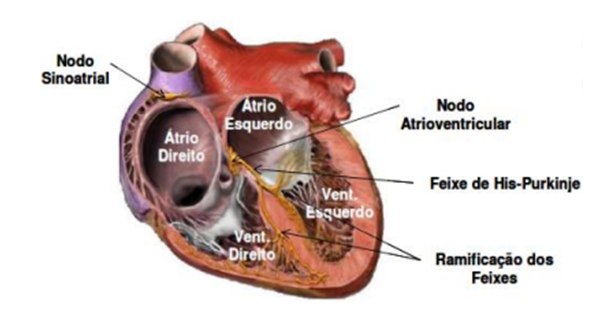
\includegraphics[width=.5\textwidth]{Figuras/cor.png}
            \vspace*{\fill} 
            \begin{quote} 
            \centering 
            Fonte: \cite{ronald} 
            \end{quote}
            \vspace*{\fill}
			\label{fig:ramcor}
\end{center}
\end{figure}

O sangue passa do átrio direito para o ventrículo direito por meio da valva tricúspide e do lado do átrio esquerdo para o ventrículo por meio da valva mitral ou conhecida como valva bicúspide. O período de contração ou bombeamento ventricular é denominado sístole enquanto a fase de relaxamento é chamada diástole. Esse sistema de contrações rítmicas é precedido por eventos elétricos coordenados e intrínsecos ao coração, responsáveis em gerar os potenciais elétricos do eletrocardiograma, que são produzidos por células eletricamente excitáveis.

A ativação elétrica inicia num ponto do átrio direito denominado de nódulo sinoatrial (AS). O nódulo sinoatrial atua de forma independente regulando a frequência cardíaca. Entretanto, ele é influenciado por sinais neurológicos e hormonais, interferindo na frequência de batimento cardíaca \cite{silva}.

As fibras do nódulo sinusal ou sinoatrial possui o diâmetro entre 3 a 5 micrômetros enquanto as fibras atriais musculares que as contornem possui de 10 a 15 micrômetros de diâmetro. Essas fibras estão conectadas de modo direto, ou seja, qualquer potencial de ação que se inicie no nódulo se difunde imediatamente para a parede do músculo atrial \cite{guyton}.

\subsection{O CICLO CARDIÁCO}

\hspace*{0.8cm}O ciclo cardíaco corresponde ao intervalo do início de um batimento cardíaco até o início do próximo batimento. O responsável por fornecer o ciclo cardíaco é o nodo sinoatrial localizado na parede lateral superior do átrio direito, próximo a abertura da veia superior que gera o potencial de ação que se propaga imediatamente pelo os átrios e aos ventrículos através do feixe A-V com duração acima de $0,1$s. Em função desse retardo os átrios se contraiam antes dos ventrículos, portanto, os átrios bombeiam o sangue para os ventrículos antes da forte contração ventricular.\cite{guyton}.

O nodo atrioventricular tem como função retardar a passagem do impulso dos átrios para os ventriculos. No periodo que ocorre a ativação do nodo atrioventricular, o impulso pecorre até o  o feixe de His-Purkinje que os divide em dois ramos direito e esquerdo de His e se ramificam pela as fibras de Purkine, responsável pela despolarização e contração do miocárdio ventricular.  

A Figura \ref{fig:card} apresenta a característica dos eventos fornecidos pelo os ciclos cardíacos, para o lado esquerdo do coração. No ciclo cardíaco é possível extrair informação de pressão aórtica, pressão atrial, pressão ventricular, volume ventricular, fonocardiograma e por fim o eletrocardiograma que será a base desse trabalho.

\begin{figure}[H]
\begin{center}
			\caption{Eventos do Ciclo Cardíaco}
			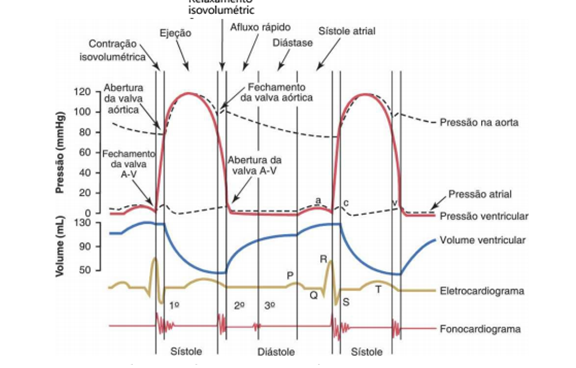
\includegraphics[width=.5\textwidth]{Figuras/ecc.png}
            \vspace*{\fill} 
            \begin{quote} 
            \centering 
            Fonte: \cite{guyton}
            \end{quote}
            \vspace*{\fill}
			\label{fig:card}
\end{center}
\end{figure}


\subsection{O ELETROCARDIOGRAMA}

\hspace*{0.8cm}O eletrocardiograma é um sinal obtido através da aquisição dos sinais elétricos localizados no musculo cardíaco. A aquisição do sinal é obtida através da distribuição de sensores em ponto especifico sobre a pele utilizando eletrodos. O registro da atividade cardíaca é fornecido através do eletrocardiógrafo que fornece e registra gráficos dos impulsos elétricos que estimulam a contração do coração em função do tempo \cite{thaler}.

A Figura \ref{fig:ecg} mostra um eletrocardiograma típico com a identificação das diversas ondas, tradicionalmente denominadas P, Q, R, S e T. A onda P é a primeira onda do sinal do eletrocardiograma e representa a despolarização dos átrios direito e esquerdo sua amplitude é normalmente menor que 300$\mu$V, e a sua duração é inferior a 120ms. Essa onda possui espectro abaixo de 10-15 Hz \cite{sornmo}.

\begin{figure}[!htb]
\begin{center}
			\caption{Característica do sinal do eletrocardiograma}

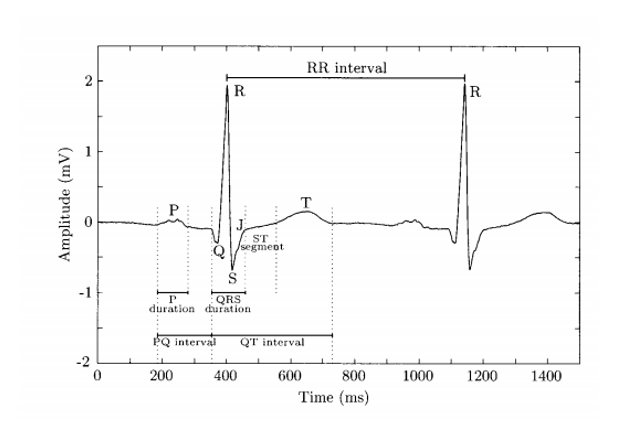
\includegraphics[width=.5\textwidth]{Figuras/ecg1.PNG}
            \vspace*{\fill} 
            \begin{quote} 
            \centering 
            Fonte: \cite{sornmo}
            \end{quote}
            \vspace*{\fill}
			\label{fig:ecg}
\end{center}
\end{figure}



O complexo QRS é caracterizado pela despolarização dos ventrículos esquerdo e direito em torno de 70ms a 110ms. Essa composição de sinal é analisada através das ondas Q, R e S. Esse complexo possui a maior amplitude em torno de 2mV a 3mV, e é a forma de onda que é analisada primeiro em aspectos computacionais devido a sua amplitude ser maior que as outras  \cite{sornmo}. 

O segmento ST é caracterizado pela a despolarização dos ventrículos direito e esquerdo. Esse segmento inicia no final da onda S conhecido como ponto J até a extremidade da onda T. Já o intervalo PQ corresponde ao tempo necessário para que o impulso elétrico se propague a partir do nódulo sino-atrial para os ventrículos é dependente da frequência cardíaca \cite{sornmo}.

O intervalo RR corresponde ao comprimento de um ciclo cardíaco que representa o intervalo entre dois batimentos cardíacos e é usado para determinar arritmias irregulares. O intervalo QT apresenta o tempo do começo da despolarização até a repolarização dos ventrículos. Este intervalo varia com a frequência cardíaca o qual em taxas mais rápidas o mesmo torna-se reduzido. Por fim, a onda T representa a repolarização ventricular com duração de 300ms e é iniciada após o complexo QRS e as vezes é seguida por onda conhecida como U. A característica é arredonda e está associada a um único pico positivo \cite{sornmo}.


\subsection{DERIVAÇÕES ELETROCARDIOGRÁFICAS}
\hspace*{0.8cm} A derivação é uma linha que une eletricamente os eletrodos ao aparelho de eletrocardiograma. As derivações eletrocardiográficas são divididas em derivação bipolar, subdivididas em derivação I, derivação II e derivação III e as derivações unipolares que são divididas em V1, V2, V3, V4, V5, V6 as como aVR, aVL, aVF.

\subsubsection{As Três Derivações Bipolares}

\hspace*{0.8cm}A caracterização do vetor resultante da ativação elétrica cardíaca é feita através de parâmetros utilizando pares de eletrodos situados em pontos diferentes do corpo humano. Cada parâmetro resultante das medições é chamado de derivação, representando assim uma projeção desse vetor e espelhando a atividade elétrica cardíaca em uma região do coração \cite{webster}. Na aquisição de sinais podem ser usadas as derivações unipolar e bipolar.

As derivações bipolares do plano frontal (DI, DII e DII) são formadas pela a combinação de um par de eletrodos, sendo um posicionado nos membros inferiores e superiores depedendo da derivação conforme a Tabela 1.


\begin{table}[H]
\centering
\caption{Posicionamento dos terminais}
\begin{center}
\begin{tabular}{|l|l|l|}
\hline
\textbf{Derivações Bipolares} & \textbf{Terminal +} & \textbf{Terminal -} \\ \hline
\textbf{Derivação I}          & Braço esquerdo      & Braço direito       \\ \hline
\textbf{Derivação II}         & Perna esquerda      & Braço direito       \\ \hline
\textbf{Derivação III}        & Perna esquerda      & Braço esquerdo      \\ \hline
\end{tabular}
\end{center}
 \vspace*{\fill} 
            \begin{quote}
            \centering 
            \vspace{12pt}Fonte: Elaborada pela autora 
            \end{quote}
            \vspace*{\fill}
			\label{fig:ramcor}
\end{table}

Na Figura \ref{fig:d1} temos o posicionamento específico de cada terminal (positivo e negativo) do eletrocardiógrafo. Para a primeira derivação o terminal negativo é conectado no braço direito, enquanto o negativo posicionado no braço direito. A derivação II é resultante da combinação do terminal positivo alojado na perna esquerda e o terminal negativo alojado no braço direito e a última derivação é consequente ao alojamento do terminal positivo na perna esquerda enquanto o negativo no braço esquerdo. As derivações bipolares de cada resultante da derivação podem ser observadas na  Figura \ref{fig:d2}. O primeiro gráfico representa a derivação I, o segundo a derivação II e por fim a derivação III.

\begin{figure}[!htb]
\begin{center}
			\caption{Derivações bipolares no plano frontal}
			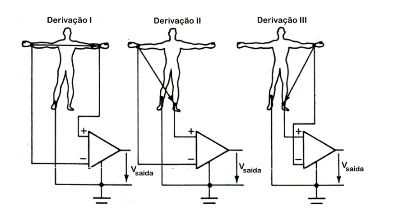
\includegraphics[width=.5\textwidth]{Figuras/d1.PNG}
            \vspace*{\fill} 
            \begin{quote} 
            \centering 
            Fonte: \cite{ebah}
            \end{quote}
            \vspace*{\fill}
			\label{fig:d1}
\end{center}
\end{figure}




\begin{figure}[H]
\begin{center}
			\caption{Comportamento da forma de onda da Derivação I, II e III}
			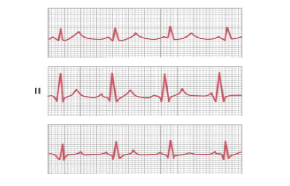
\includegraphics[width=.5\textwidth]{Figuras/d2.PNG}
            \vspace*{\fill} 
            \begin{quote} 
            \centering 
            Fonte: \cite{guyton}
            \end{quote}
            \vspace*{\fill}
			\label{fig:d2}
\end{center}
\end{figure}
\subsubsection{Derivações Torácicas}
\hspace*{0.8cm} As derivações torácicas conhecida também como derivações precordiais são obtidas através do posicionamento de seis eletrodos situados na parede anterior ao tórax diretamente no coração. O posicionamento dos eletrodos geram as seis derivações que são nominadas como derivação V1, V2, V3, V4, V5 e V6, as respectivas derivações medem a diferença de potencial (ddp) entre o torax e o centro elétrico do coração. 
As derivações vão desde de V1 localizado no espaço intercostal direito até a derivação V6, localizado no espaço intercostal esquerdo sendo mostrado na Figura \ref{fig:dop}.

\begin{figure}[H]
\begin{center}
			\caption{Posicionamentos dos seis eletrodos na região torácica}
			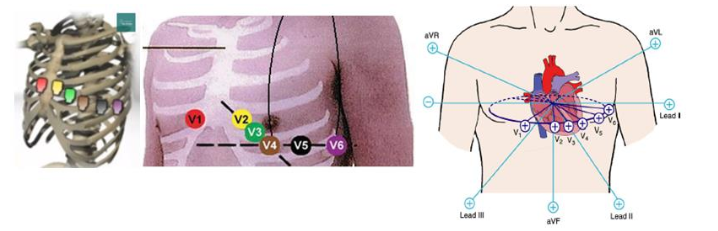
\includegraphics[width=1\textwidth]{Figuras/v6.PNG}
            \vspace*{\fill} 
            \begin{quote} 
            \centering 
            Fonte: \cite{ronald}
            \end{quote}
            \vspace*{\fill}
			\label{fig:dop}
\end{center}
\end{figure}


Na Figura \ref{fig:d2} é possível observar a forma de onda de cada derivação do plano horizontal na ordem de V1 a V6. O eletrodo da derivação V1 avalia o lado direito do coração, localizado no quarto espaço intercostal direito, justaestemal, a derivação V2 avalia o lado direito do coração localizado no quarto espaço intercostal esquerdo, justamental, a derivação V3 avalia uma região intermediária entre V2 e V4, a derivação V4 localiza-se no quinto espaço intercostal esquerdo na linha hemiclavicular, a derivação V5 entre o 5º espaço intercostal esquerdo na linha axilar anterior e a derivação V6 localiza-se no quinto espaço intercostal esquerdo na linha axilar média \cite{ronald}.

\begin{figure}[H]
\begin{center}
			\caption{Comportamento das forma de ondas da Derivação V1, V2, V3, V4, V5 e V6.}
			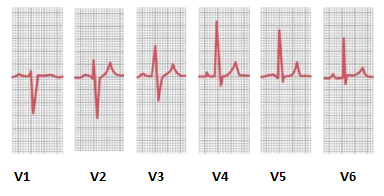
\includegraphics[width=.5\textwidth]{Figuras/DEV.PNG}
            \vspace*{\fill} 
            \begin{quote} 
            \centering 
            Fonte: \cite{guyton}
            \end{quote}
            \vspace*{\fill}
			\label{fig:d2}
\end{center}
\end{figure}


\subsubsection{As Derivações Unipolares Aumentadas}


\hspace*{0.8cm}As derivações  unipolares obtêm potenciais locais, ou seja, cada derivação é obtida através do posicionamento de eletrodos exploradores. A derivação VR é obtida através do alojamento do eletrodo explorador no braço direito, a derivação VL é adquirida posicionado o eletrodo no braço esquerdo e quando o eletrodo é colocado na perna esquerda tem-se a derivação VF que são baseadas em um ponto conhecido como Terminal Central de Wilson (WCT), conforme apresentado na Figura \ref{fig:ab}.

As derivações unipolares aumentadas denominadas como aVR, aVL e AVF são fornecidas através de dois membros são conectados ao terminal negativo através de resistências elétricas e o terceiro membro conectado ao terminal positivo.

\begin{figure}[H]
\begin{center}
			\caption{Terminal Central de Wilson}
			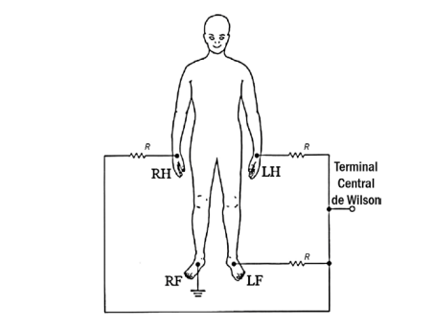
\includegraphics[width=.5\textwidth]{Figuras/WCT.PNG}
            \vspace*{\fill} 
            \begin{quote} 
            \centering 
            Fonte: \cite{webster}
            \end{quote}
            \vspace*{\fill}
			\label{fig:ab}
\end{center}
\end{figure}
O tipo de configuração de resistência mostrada na Figura \ref{fig:ab} tende a reduzir a amplitude do sinal. Para o aumento da amplitude o  circuito é modificado para a geração da derivação unipolar aumentada (aVR, aVL e aVF) que são as derivações que são mostradas em monitores cardíacos.

A Figura \ref{fig:aca} representa a configuração do terminal de Wilson com a resistência elétrica modificada para gerar o aumento da amplitude. Neste tipo de configuração, dois membros são conectados, por meios das resistências elétricas, ao terminal negativo e o terceiro membro no terminal positivo para a derivação aVL o terminal positivo precisa está conectado ao braço esquerdo e a ultima derivação aumentada denominada AVF precisa que a perna esquerda esteja conectado ao terminal positivo \cite{guyton}. 

\begin{figure}[!htpb]
\begin{center}
			\caption{Derivações unipolares a) aVR, b)aVL, c) aVF }
			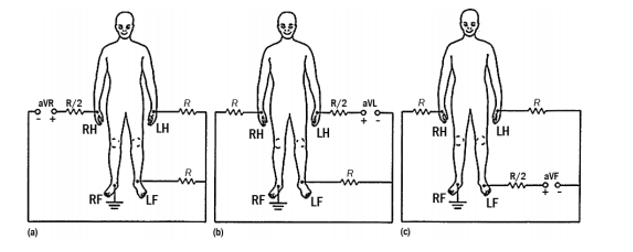
\includegraphics[width=.5\textwidth]{Figuras/avr.PNG}
            \vspace*{\fill} 
            \begin{quote} 
            \centering 
            Fonte: \cite{webster}
            \end{quote}
            \vspace*{\fill}
			\label{fig:aca}
\end{center}
\end{figure}

Para obter a derivação aVR, a resistência conectada ao eletrodo do braço direito é modificada enquanto os demais continuam com o mesmo valor. Para a geração da derivação aVL a resistência que é modificada fica conectada ao eletrodo do braço esquerdo e para a derivação aVF a resistência é modificada no eletrodo que é conectado a perna esquerda. Esse arranjo serve para aumentar a amplitude de cada derivação unipolar aumentada (aVR, aVL e aVF), essas derivações tem a característica de formas de ondas mostrada na Figura \ref{fig:aba}, a primeira a forma de onda representa a primeira unipolar aumentada aVR, a segunda aVL e a terceira aVF.

\begin{figure}[!htpb]
\begin{center}
			\caption{Registro das três derivações unipolares aumentadas}
			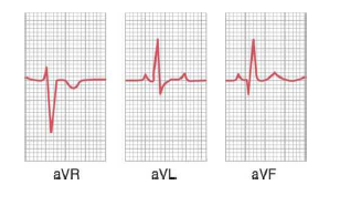
\includegraphics[width=.5\textwidth]{Figuras/tres.PNG}
            \vspace*{\fill} 
            \begin{quote} 
            \centering 
            Fonte: \cite{guyton}
            \end{quote}
            \vspace*{\fill}
			\label{fig:aba}
\end{center}
\end{figure}

Na Tabela 2 apresenta as relações matemáticas para obtenção das derivações eletrocardiográficas a partir do posicionamento dos eletrodos  posicionandos nos membros inferiores e superiores (LA - braço esquerdo, LL - braço direito, RA- perna esquerda e RL- perna direita) e dos eletrodos posicionando na região torácica (v1, v2, v3, v4, v5 e v6).  

\begin{table}[H]
\centering
\caption{Representação Algebrica através do posicionamento dos eletrodos }
\begin{center}
\begin{tabular}{|l|l|l|ll}
\cline{1-3}
Tipo de Derivação                                                                       & Eletrodos Utilizados   & Definição                                                                                                                                                             &  &  \\ \cline{1-3}
\begin{tabular}[c]{@{}l@{}}Bipolar \\ ou \\ Derivação de membros Einthoven\end{tabular} & LA, RA, LL, RL         & \begin{tabular}[c]{@{}l@{}}I= LA-RA\\ II = LL-RA\\ III = LL-LA\end{tabular}                                                                                           &  &  \\ \cline{1-3}
Aumentadas                                                                              & LA, RA, LL, RL         & \begin{tabular}[c]{@{}l@{}}aVR= RA-1/2(LA+LL)\\ aVL =LA-1/2(LL+RA)\\ aVF = LL-1/2(LA+RA)\end{tabular}                                                                 &  &  \\ \cline{1-3}
Unipolar                                                                                & V1, V2, V3, V4, V5, V6 & \begin{tabular}[c]{@{}l@{}}V1 = v1-(RA+LA+LL)/3\\ V2=v2-(RA+LA+LL)/3\\ V3=v3-(RA+LA+LL)/3\\ V4=v4-(RA+LA+LL)/3\\ V5=v5-(RA+LA+LL)/3\\ V4=v6-(RA+LA+LL)/3\end{tabular} &  &  \\ \cline{1-3}
\end{tabular}
\end{center}

 \vspace*{\fill} 
            \begin{quote}
            \centering 
            \vspace{12pt}Fonte: Elaborada pela autora 
            \end{quote}
            \vspace*{\fill}
			\label{fig:ramcor}
\end{table}            

\subsection{O TRIÁNGULO DE EINTHOVEN }

\hspace*{0.8cm}O triângulo de Einthoven é uma representação vetorial em torno do coração que permite estudar as forças eletromotrizes geradas pelo coração. Esse representação fornece  diferença de potencial entre eletrodos localizados em diversos membros sobre a pele conhecidas como derivação I, II e III, caso os potenciais elétricos de duas das três derivações bipolares forem conhecidos e a terceira pode ser determinada matemáticamente a partir das duas primeiras. Na Figura \ref{fig:jup} temos o triângulo de Einthoven.

\begin{figure}[!htpb]
\begin{center}
			\caption{Triângulo de Einthoven.}
			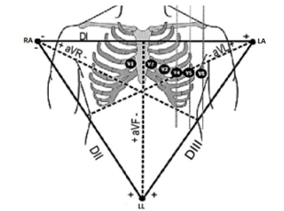
\includegraphics[width=.5\textwidth]{Figuras/triangulo.png}
            \vspace*{\fill} 
            \begin{quote} 
            \centering 
            Fonte: \cite{souza}
            \end{quote}
            \vspace*{\fill}
			\label{fig:jup}
\end{center}
\end{figure}

A derivação I registra a diferença de potencial entre o braço direito e braço esquerdo, a derivação II entre o braço direito e perna esquerda e derivação III entre o braço esquerdo e a perna direita. 

A Figura \ref{fig:jup} representa a figura geométrica do Triângulo de Einthoven. O braco direito e esquerdo e a perna esquerda formam os ápices do triângulo que envolve o coração. Os ápices superiores representam os pontos localizados no braço esquerdo e braço direio e o ápice inferior representa a perna esquerda se conecta aos dois pontos, a ligação entre todos os apices fornecem o Triângulo de Einthoven.

\subsection{ELETRODOS}

\hspace*{0.8cm}Os eletrodos são sensores que têm como função medir e registrar os biopotenciais através da interface fornecida pelo corpo humano e o circuito de aquisição. Os eletrodos podem ser classificados como eletrodos invasivos e não invasivos. Os eletrodos invasivos são inseridos internamente ao corpo para a detecção de biopotenciais, e também são conhecidos como subcutâneos. Os eletrodos não invasivos são utilizados para detectar biopotenciais a partir da superfície do corpo \cite{vier}.

Normalmente, os eletrodos mais utilizados para monitoração do eletrocardiograma são do tipo autoadesivos constituídos por gel sólido de cloreto de potássio, uma capa plástica para manter a umidade do gel, pino de aço inox, contra pino de prata cloreto de potássio, papel protetor sendo o contato elétrico com a pele \cite{Site22}. Na Figura \ref{fig:eletrodo} temos um exemplo de eletrodo do tipo não invasivo, comum em sistemas de ECG.
%http://www.fibracirurgica.com.br/eletrodo-descartavel-espuma-2223brq-pacote-c-50-unidades-3m/p

\begin{figure}[!htpb]
\begin{center}
			\caption{Eletrodos do tipo não invasivo.}
			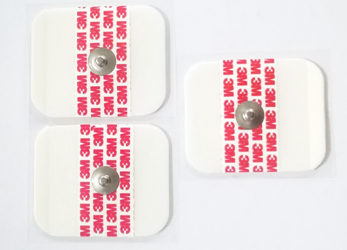
\includegraphics[width=.5\textwidth]{Figuras/eletrodo.png}
            \vspace*{\fill} 
            \begin{quote} 
            \centering 
            Fonte: Elaborada pela autora
            \end{quote}
            \vspace*{\fill}
			\label{fig:eletrodo}
\end{center}
\end{figure}

\subsection{INTERFERÈNCIA EM SINAIS DE ECG}

\hspace*{0.8cm}O sinal ECG é sensível a interferências, principalmente devido a característica deste sinal possui pequena amplitude, por volta de 1mVpp. No sistema de captação do sinal ECG utiliza no mínimo dois eletrodos exploratórios e um de referência.

O tipo de interferência mais comum em sistema de aquisição de sinais biológicos é oriundo a frequência da rede elétrica e induzido por meios de acoplamentos entre o comum do circuito eletrônico, ou terra, e a rede elétrica que alimenta o dispositivo  pode variar dependendo do país sendo  50Hz e 60Hz.

A interferência pode ser inserida ao sinal devido a diferença de impedância entre os eletrodos, o que resulta em desbalanceamento nas tensões de modo comum e as converte em tensões diferenciadas, sendo assim amplificadas. Esse fenômeno é nomeado de efeito de divisor de potencial.\cite{webster}

A Figura \ref{fig:tri}  representa a interferência de 60 Hz no sinal do eletrocardiograma. O sinal em azul representa em condições ideais e o vermelho com a interferência da frequência.

\begin{figure}[!htb]
\begin{center}
			\caption{Sinal ECG com interferência devido a rede elétrica}
			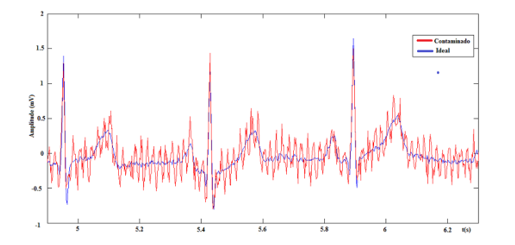
\includegraphics[width=.5\textwidth]{Figuras/freq.PNG}
            \vspace*{\fill} 
            \begin{quote} 
            \centering 
            Fonte: \cite{android}
            \end{quote}
            \vspace*{\fill}
			\label{fig:tri}
\end{center}
\end{figure}

Para solucionar problemas com interferências no sinal do ECG são aplicados vários tipos de filtros sendo filtro passa- baixa, passa – alta, notch e casado.
\begin{itemize}
\item Filtro passa- alta: Aplicado para remoção do sinal base.
\item Filtro passa – baixa: Remoção do ruído muscular.
\item Filtro Notch:  Remoção do ruído de 60Hz da rede elétrica.
\item Filtro Casado: Utilizado para comparar uma forma de onda com outra utilizada como onda padrão. Esse tipo de filtro é fundamental para que seja encontrado o completo QRS e seja, portanto, uma análise para possível detecção de anomalia. 

\end{itemize}


%Chamda de site \cite{wiki}.

\subsection{CIRCUITO DE AQUISIÇÃO}
\hspace*{0.8cm} O circuito de aquisição é responsável em adquirir o sinal de ECG. A aquisição do sinal é de extrema importância, pois é a primeira etapa do sistema de captação e transmissão de sinais de ECG. Este circuito é composto basicamente por um amplificador de instrumentação específico para sinais de ECG, devido a sua baixa energia \cite{pds}.


O amplificador de instrumentação é um circuito integrado e geralmente constituído por três amplificadores operacionais, sendo aplicado para medir sinais analógicos de baixa amplitude que requer exatidão. A Figura \ref{fig:cir} apresenta a estrutura deste amplificador. Pode se observar que este possui dois estágios: um estágio de entrada, constituído por dois amplificadores não-inversores e o segundo estágio formado por um amplificador subtrator \cite{veloso}. 

\begin{figure}[!htb]
\begin{center}
			\caption{Estrutura característica de um amplificador de instrumentação.}
			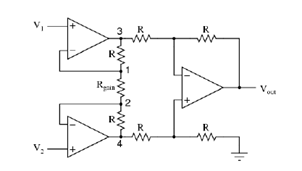
\includegraphics[width=.5\textwidth]{Figuras/circuito.png}
            \vspace*{\fill} 
            \begin{quote} 
            \centering 
            Fonte: \cite{sugi}
            \end{quote}
            \vspace*{\fill}
			\label{fig:cir}
\end{center}
\end{figure}

Após a aquisição do sinal, o sinal de ECG pode ser enviado para outros tipos de circuitos a depender do sistema, como por exemplo, circuitos de amplificação de segundo estágio e filtragem e circuitos de modulação.

\subsection{FILTROS ATIVOS}
\hspace*{0.8cm}Os filtros são circuitos eletrônicos que executam o processamento de sinais especificamente atenuando frequências indesejadas de sinais de entradas de um circuito, tem como característica permitir a passagem ou suprimir sinais com certas frequências dependendo da topologia empregada. Um circuito de filtro ativo pode ser construído utilizando componentes tais como: amplificadores operacionais, transistores, resistores, capacitores.

Um filtro que permite a passagem de sinais de tensões e corrente somente em frequências abaixo de certo limite, atenuando os sinais cuja a frequência ultrapassar esse valor é chamado de filtro passa-baixa. Um filtro que permite a passagem de sinais acima de uma frequência de corte é um filtro passa-alta. Quando um circuito apresenta a passagem de sinal acima de uma frequência de corte e abaixo de outra frequência de corte, é chamado de filtro passa-banda \cite{boy}.

\subsection{CONVERSOR ANALÓGICO/ DIGITAL}

\hspace*{0.8cm}Um conversor analógico-digital recebe uma tensão analógica de entrada e posteriormente produz um sinal digital de saída correspondente a entrada analógica. Para conversão do sinal analógico é realizado a amostragem do sinal. As principais técnicas de conversão são a paralelo (também conhecida como flash), contador de rampa contínuo e aproximação sucessivas. Suas características desejadas estão na precisão e tempo máximo de conversão \cite{digi}.

Alguns circuitos integrados (CIs) implementam conversores analógico-digital e podem ser utilizados utilizando algum tipo de protocolo. Um deles é o MCP3008, que é um CI de 16 pinos, sendo 8 entradas analógicas com 6 entradas de sinais de controle, com saída utilizando o protoloco  de comunicação SPI (\textit{Serial Peripheral Interface}). Esse protocolo permite a comunização utilizando a interconexão de dispositivos ou chips de forma que estes troquem informação entre si.
%http://www.alan.eng.br/disc_microprocessadores/pratica8_spi.pdf


\subsection{CLIENTE-SERVIDOR}

\hspace*{0.8cm}Os dipositivos em geral, utilizam protocolos de comunicação, sendo os principais: IP (\textit {Internet Protocol}), TCP (\textit {Transmission Control Protocol}) e HTTP, (\textit{Hypertext Transfer Protocol}). Estes são protocolos de padronização que possibilitam a troca de informação entre si de diferentes equipamentos. Esses protocolos são usados na transferência de informações e são também aplicado na arquitertura cliente-servidor.

\hspace*{0.8cm}Esse tipo de arquitetura é caracterizada em dois nível chamada cliente-servidor, e funciona da seguinte maneira: o cliente socilita um recurso e o servidor responde com a solicitação do cliente, utilizando  a internet como principal meio de comunicação. A Figura \ref{fig:cli} representa a estrutura do processo cliente servidor, no qual o cliente solicita e o servidor responde a solicitação do cliente.

O termo cliente-servidor refere-se quando se tem dois ou mais computadores interagindo de modo que um oferece serviço a outro, permite ao usuário acessar a informação e serviços em qualquer lugar. 
\begin{itemize}
\item Cliente: Conhecido como ``front-end'' ou ``WorkStation'' é um recurso o qual usuário interage com o usuário através de uma interface gráfica, ou não, permitindo consultas de dados, manipulação  de tela, entrada e validação de dados, gerenciamento de som e áudio e entre outras funções. Normalmente o cliente é dedicado a sessão do usuário solicitando serviços, iniciando e finalizando a sessão.
\item Servidor: Respondem as solicitações gerada pela o cliente, é um processo contínuo, oferecendo serviços quando solicitado pelo o cliente,integra serviços de armazenamento, acesso, organiza os dados, atualiza os dados, gerencia os recursos compartilhados e entre outros serviços. 

\end{itemize}

\begin{figure}[H]
\begin{center}
			\caption{Estrutura Cliente-Servidor}
			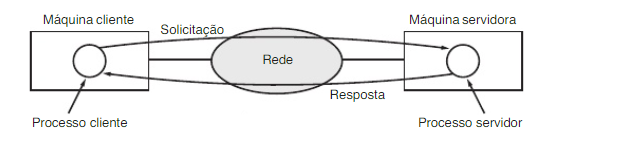
\includegraphics[width=.9\textwidth]{Figuras/servidor.PNG}
            \vspace*{\fill} 
            \begin{quote} 
            \centering 
            Fonte: \cite{tanen}
            \end{quote}
            \vspace*{\fill}
			\label{fig:cli}
\end{center}
\end{figure}


\newpage

\section{MÓDULO DE AQUISIÇÃO E TRANSMISSÃO DE SINAIS ELETROCARDIOGRÁFICO}

\hspace*{0.8cm}Este capítulo aborda o desenvolvimento do módulo de aquisição de sinais ECG, como também o circuito de conversão analógico e digital e tranmissão desses dados via Wi-Fi para um computador. Além disso, esse capítulo aborda aspectos da placa de aquisição de sinais, desenvolvimento do software para transmissão do sinal, responsável por receber os dados e exibi-los na tela do computador. 

Uma vez que o sinal de ECG possui a amplitude em escala de milivolts é necessário um mecanismo para que seja realizado o condicionamento deste sinal. O circuito responsável por tratar o sinal é composto de amplificadores, filtros e conversores A/D acoplados com o Raspberry Pi 3. 

O desenvolvimento do projeto consistiu em duas etapas: a primeira etapa do projeto de pesquisa, consistiu na aquisição, leitura e  teste do hardware, composto pela a Placa End Front-End e o MCP3008. Nesta estapa foram parametrizados as limitações dos componentes, tratamento e visualização dos sinais que compõe o eletrocardiograma. Nesta fase utilizou-se para a simulação o simulador ECG 12 derivações HS-15, da RQ Mediq, que representam a cópia autêntica do sinal gerado pelo o corpo humano.


A segunda parte do projeto consistiu na transferência dos dados para um computador, utilizando o protocolo de comunicação em rede (TCP/IP). Nesta etapa foram definidos os protocolos e a linguaguem de programação, com a finalidade de transferir  as amostras geradas pelo o simulador de sinais ao computador, transpondo dessa maneira as amostras em um determinado espaço de tempo em forma de gráfico, tendo como característica principal sinais digitais de ECG compostos pelas as ondas P, complexo QRS e a onda T. 

A Figura \ref{fig:pap} representa as etapas desde a aquisição dos sinais através dos eletrodos, cabos e circuito de aquisição até a transferência ao usuário utilizando conversores, linguagem de programação embarcado no Raspberry Pi. 
    
\begin{figure}[H]
\begin{center}
			\caption{Diagrama do trabalho  desenvolvido.}
			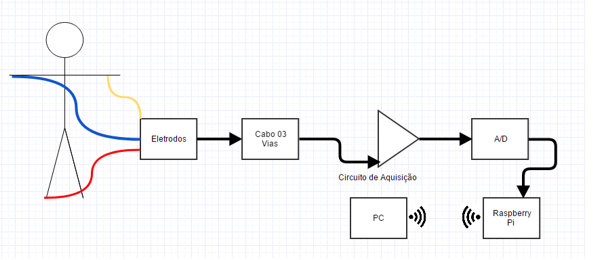
\includegraphics[width=.9\textwidth]{Figuras/pac.PNG}
            \vspace*{\fill} 
            \begin{quote} 
            \centering 
            Fonte: Elaborada pela autora
            \end{quote}
            \vspace*{\fill}
			\label{fig:pap}
\end{center}
\end{figure}

Lista de materiais do projeto


\begin{itemize}
\item 01 AD8232
\item 01 Simulador de ECG Handy Sim HS-15
\item 01 MCP3008
\item 01 Raspberry Pi 3
\item 01 Cabo HDMI
\item 01 Cabo paciente de 03 vias.
\item 03 eletrodos auto adesivos
\item 01 Carregador 5,1 volts/2,5 Ampere
\item 01 Computador
\item 01 CABO PACIENTE ECG 5 VIAS AE-0H002-0
\item Tornado versão: 4.5.2
\end{itemize}

\subsection{MÓDULO DE AQUISIÇÃO DE SINAIS ECG}
\hspace*{0.8cm} O módulo de aquisição de sinais ECG é composto basicamente por um componente AD8232, constituído basicamente por amplificador  instrumentação, um filtro de condicionamento do sinal e um aplificador de realimentação ou um circuito de perna direita cuja função desse componente é obter e filtrar os sinais de eletrocardiograma integrado em único capsulamento, comercializado pelo o fabricante Analog Devices.

\subsubsection{Placa ECG Front-End}
\hspace*{0.8cm}A placa de ECG escolhida é aplicada para  tratamento e condicionamento de pequenos sinais que compõem os sinais  ECG, projetado para filtrar, extrair e amplificar pequenos sinais cardíacos, é da empresa SparkFun, baseada no CI AD8232 da Analog Devices, é composto por 20 pinos e internamente este pinos são entrada e saída de amplificadores de instrumentação e operacional aplicados a este componente, sendo detalhado na Figura \ref{fig:core}.

O CI AD8232 possibilita ao usuário implementar várias funções como o uso de filtros para eliminar artefatos de movimentos, ou seja, anormalidades que não resultam da atividade elétrica do coração, amplificadores operacional permite filtro passa-baixa para remover o ruído adicional, filtro passa alta para eliminar sinais provenientes do movimento muscular e do eletrodo.

A Figura \ref{fig:circ} representa a característica externa e interna do AD8232 e as respectivas pinagens composto por 20 pinos. Internamente possui um amplificador de instrumentação (IA), um amplificador operacional (A1), um aplificador de unidade perna direita (A2) e um buffer da entrada de referência (A3).

A configuração interna da placa da Sparkfun é projetada para realizar o monitoramento da forma de onda composto pelas as ondas P, complexo QRS e a onda T. Esse sinal possui baixa amplitude logo é susceptível a ruídos, portanto, para obter o sinal sem distorção é acoplado  filtro passa-alta com dois pólos em 0,5 Hz seguido de um filtro passa-baixa com dois-pólos em 40 Hz. Um terceiro circuito de alimentação é conduzido para uma rejeição de modo comum.

Especificação:
\begin{itemize}
\item Tensão de Operação 3.V.
\item Saída analógica
\item Peso 4g
\item 03 Pinos de Entrada (RA, LA e RL)
\item Temperatura de Funcionamente 40 a 55.%Não seicolocar o grau
\item Led indicador
\item Tamanho 4mm x 4mm

\end{itemize}

\begin{figure}[H]
\begin{center}
			\caption{Pinagem do AD8232}
			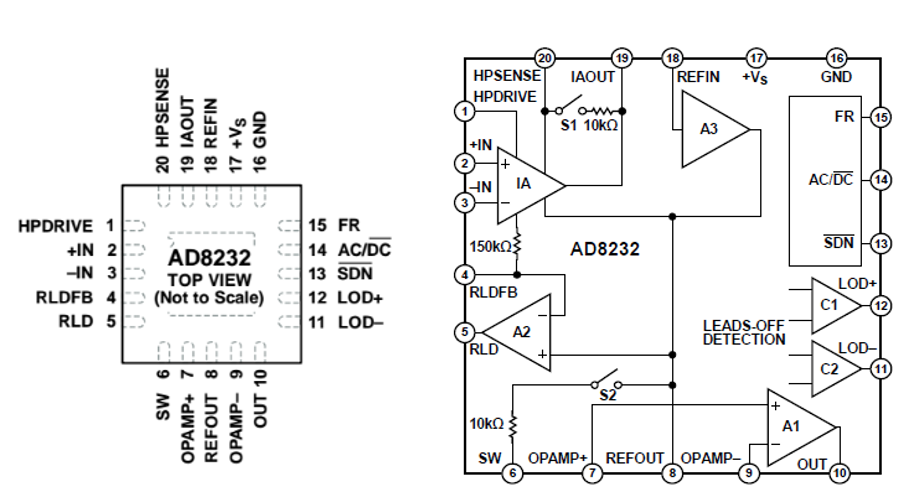
\includegraphics[width=.9\textwidth]{Figuras/adc.PNG}
            \vspace*{\fill} 
            \begin{quote} 
            \centering 
            Fonte: \cite{analogic}
            \end{quote}
            \vspace*{\fill}
			\label{fig:core}
\end{center}
\end{figure}

A placa de ECG Front-End utilizada é da empresa Sparkfun e possui internamente o AD8232, resistores e capacitores de precisão. Os pinos RA, LA e RL são respectivamente do braço direito, braço esquerdo e perna direita. Externamente possui um led indicador que pulsa na frequência do ciclo cardíado além de outras 6 saídas que são de aterramento do circuito (GND), tensão de alimentação (3,3V), saída analógica (OUTPUT), detectores de eletrodo (LO-/LO+) e desligamento (SDN), demonstrado na Figura \ref{fig:circ}.

\begin{figure}[H]
\begin{center}
			\caption{Placa ECG}
			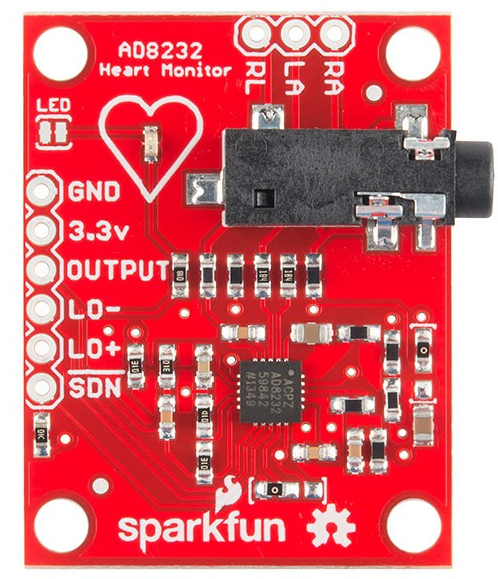
\includegraphics[width=.5\textwidth]{Figuras/pc.PNG}
            \vspace*{\fill} 
            \begin{quote} 
            \centering 
           Fonte: \cite{analogic}
            \end{quote}
            \vspace*{\fill}
			\label{fig:circ}
\end{center}
\end{figure}
Esse componente não possui conversor analógico digital, porém o mesmo permite que integre outros componentes através da saída (OUTPUT). O componente escolhido e utilizado para converter o sinal em digital é chamado de MCP3008 que será abordado na Subseção \ref{sec:conversorAD}.

\subsubsection{Conversor Analógico Digital}\label{sec:conversorAD}

\hspace*{0.8cm}O MCP3008 é um conversor analógico digital programável que opera na faixa de 2,7V a 5,5V. A comunicação com os dispositivos é realizada usando
interface serial simples compatível com o protocolo SPI.

Esse componente possui 8 entradas analógicas do canal CH0 ao CH7 e 8 pinos configuráveis. Esses pinos são conhecidos como VDD, VREF, AGND, CLK, DOUT, DIN, CS/SHDN e DGND, detalhado na Tabela 1. Os pinos DIN, DOUT e CS/SHDN pode ser conectados a outro dispositivos com interface SPI para realizar a conversão de analógico e digital. 

A Figura \ref{fig:cadc} representa a característica externa do MCP3008 com as respectivas pinagens CH0 a CH7 e entradas analógicas: VDD, VREF, AGND, CLK, DOUT, DIN, CS/SHDN E DGND.

\begin{table}[]
\centering
\begin{center}
\caption{Descrição dos Pinos}
\label{center}
\begin{tabular}{|l|l|l|}
\hline
\multicolumn{1}{|c|}{\textbf{PINOS}} & \multicolumn{1}{c|}{\textbf{SIMBOLOGIA}} & \multicolumn{1}{c|}{\textbf{DESCRIÇÃO}} \\ \hline
1                                    & CH0                                      & Entrada Analógica                       \\ \hline
2                                    & CH1                                      & Entrada Analógica                       \\ \hline
3                                    & CH2                                      & Entrada Analógica                       \\ \hline
4                                    & CH3                                      & Entrada Analógica                       \\ \hline
5                                    & CH4                                      & Entrada Analógica                       \\ \hline
6                                    & CH5                                      & Entrada Analógica                       \\ \hline
7                                    & CH6                                      & Entrada Analógica                       \\ \hline
8                                    & CH7                                      & Entrada Analógica                       \\ \hline
9                                    & DGND                                     & \textit{Digital Ground}                 \\ \hline
10                                   & CS/SHDN                                  & \textit{Chip Select/Shutdown Input}     \\ \hline
11                                   & DIN                                      & \textit{Serial Data In}                 \\ \hline
12                                   & DOUT                                     & \textit{Serial Data Out}                \\ \hline
13                                   & CLK                                      & \textit{Serial CLK}                     \\ \hline
14                                   & AGND                                     & \textit{Analog Ground}                  \\ \hline
15                                   & VREF                                     & Tensão de Referência                    \\ \hline
16                                   & VDD                                      & + 2,5V a 5,5V                           \\ \hline
\end{tabular}
\end{center}
 \vspace*{\fill} 
            \begin{quote}
            \centering 
            \vspace{12pt}Fonte: Elaborada pela autora 
            \end{quote}
            \vspace*{\fill}
			\label{fig:ramcor}
\end{table}


\begin{figure}[H]
\begin{center}
			\caption{Conversor ADC}
			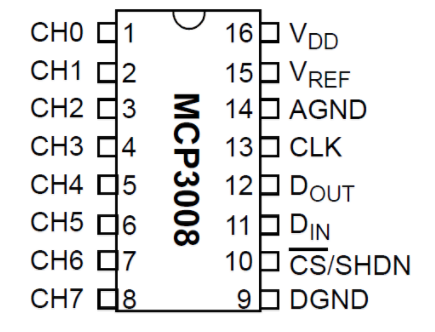
\includegraphics[width=.5\textwidth]{Figuras/mcp3008.PNG}
            \vspace*{\fill} 
            \begin{quote} 
            \centering 
           Fonte: \cite{analogica}
            \end{quote}
            \vspace*{\fill}
			\label{fig:cadc}
\end{center}
\end{figure}

Característica:

\begin{itemize}
\item ADC de 10 bits
\item 8 canais
\item Interface SPI
\item Taxa de amostragem: 200kSPS
\item Tensão de alimentação 2,7 V a 5,5 V
\item DIP de 16 pinos
\item Tempo de conversão %10μs
\item Corrente de suprimento: %425μA

\end{itemize}

\subsubsection{Raspberry Pi 3}

\hspace*{0.8cm}O Raspberry Pi é um microcomputador com tamanho equivalente a um cartão de crédito, com hardware livre, criado com o intuito de disseminar o ensino de programação para jovens e crianças. Seu custo está em torno de 10 a 35 dólares e é desenvolvido pela Raspberry Pi Foundation, uma instituição sem fins lucrativos do Reino Unido.
% https://www.raspberrypi.org 

Em comparação a outros sistemas similares como o Arduino, suas vantagens estão em oferecer ao usuário a possibilidade de ser programada em C++, Java e Phyton, enquanto o Arduino é baseado em C++.  Além disso, permite ao usuário executar vários programas ao mesmo tempo enquanto no Arduino só é possível apenas um por vez. O modelo que será utilizado neste trabalho é o último lançamento conhecido como Raspberry Pi 3 Model B, devido ao adaptador wireless integrado, o que permite ao usuário conexão à rede sem fio, possibilitando diversos tipos de aplicações \cite{usp}. 

Esse microcomputador é um computador em qualquer uma de suas versões existente no mercado, portanto é necessário instalar um Sistema Operacional (SO), como Linux ou Windows e recomenda-se que seja instalado a versão Debian Linux, porém existe outras versões disponíveis.  O sistema operacional é armazenado no cartão de memória SD, o qual funciona como disco rígido, localizado na parte inferior do hardware \cite{usp}.

A Figura \ref{fig:raspb} representa a vista superior da Raspberry Pi 3 e seus periféricos que permite gerenciar teclado, monitor, mouse, pen drive e entre outros periféricos utilizando as 4 portas USB. Possui 40 conectores de GPIO, conector Ethernet, saída de áudio e vídeo, conector de câmera, saída de vídeo, comunicação com redes e formas de comunicação serial e entre outros.

\begin{figure}[H]
\begin{center}
			\caption{Estrututa externa do Raspberry Pi 3}
			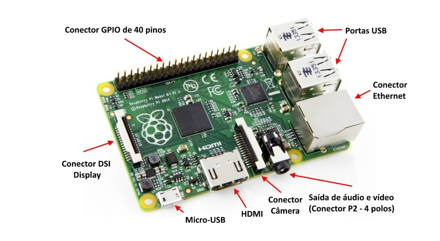
\includegraphics[width=.9\textwidth]{Figuras/RASP.PNG}
		
            \vspace*{\fill} 
            \begin{quote} 
            \centering 
           Fonte: \cite{raspb}
            \end{quote}
            \vspace*{\fill}
			\label{fig:raspb}
\end{center}
\end{figure}


Característica:

\begin{itemize}
\item Processador Bradcom BCM2837 64bit ARMv8 Cortex – A53 Quad-Core.
\item Memória RAM: 1GB
\item Adaptador Wifi 802.11n Integrado
\item Bluetooth 4.1 BLE integrado
\item Conector de video HDMI
\item 4 Portas USB 2.0
\item Conector Ethernet 
\item Interface para câmera (CSI)
\item Interface para display (DSI)
\item Slot para cartão SD
\item Conector para áudio e vídeo
\item GPIO de 40 pinos
\item Dimensão: 80 x 56 x 17mm
\end{itemize}

O Raspberry Pi não possui identificação dos pinos na placa, logo é necessário acessar o mapeamento dos pinos de acordo com Figura \ref{fig:pinosraspb}. Os pinos 2 e 4 representam pinos de alimentação de 5 Volts e especificamente essas portas não podem entrar em contato com as demais diferentemente do pino 1 e 17 que possuem saída 3,3V,  possui também 8 portas (8, 25, 6, 14, 20, 30 e 34) de aterramento (GROUND). Os pinos 3 e 4 são destinado ao uso protocolo de comunicação I2C, sendo um destinado a dados serial e outra para CLK, os pinos 8 e 10 são portas serial e utilizam protocolo RS-232 para transmissão e recepção de sinal digital. Os pinos 19, 21 ,23, 24, 26 permitem que a raspberry se comunique de forma serial Full Duplex síncrono com outro dispositivo periférico de forma bidirecional, porém o protocolo SPI precisa está implementado. As portas 26 e 28 são  portas do ID EEPROM  (\textit{Electrically-Erasable Programmable Read-Only Memory}), ou seja é um tipo de memória que pode ser programada e apagada várias vezes, através de uma tensão elétrica interna ou externa e as demais portas são pinos de GPIO que fazem envio e transmissão de sinais digitais. %ref [http://blog.fazedores.com/raspberry-pi-b-introducao-porta-gpio/]

\begin{figure}[H]
\begin{center}
			\caption{Mapeamento dos pinos do Raspberry Pi 3}
			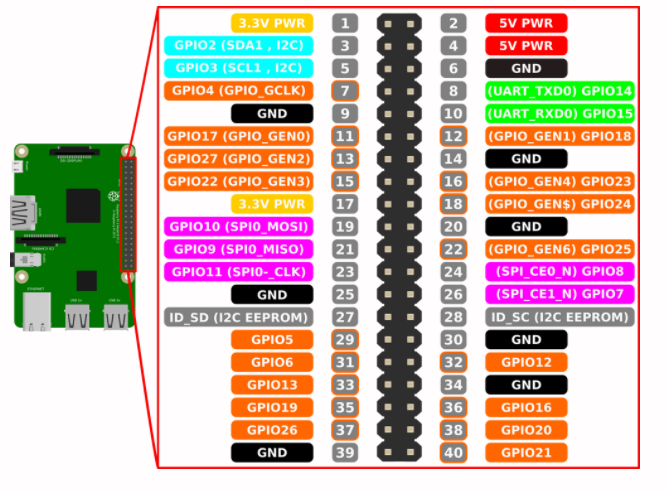
\includegraphics[width=.9\textwidth]{Figuras/pins.PNG}
			\vspace*{\fill} 
            \begin{quote} 
            \centering 
           Fonte: \cite{ras}
            \end{quote}
            \vspace*{\fill}
			\label{fig:pinosraspb}
\end{center}
\end{figure}

%fonte: https://jeremylindsayni.wordpress.com/2017/04/05/turning-gpio-pins-high-and-low-on-a-raspberry-pi-3-using-net-core-2-and-ubuntu/
\subsubsection{Cabo Paciente}
\hspace*{0.8cm} O cabo paciente é utilizado em monitores cardiacos e eletrocardiografo que auxiliam esses equipamentos a monitorar sinais ECG. O cabo utilizado é fabricado pela a empresa Dixtal Philips o qual possui certificação pela a ANVISA. O modelo utilizado para o experimento é definido como cabo paciente ECG 5 vias (AE-0H0020). Este modelo está apresentado na Figura \ref{fig:cabopaciente}.
\begin{figure}[H]
\begin{center}
			\caption{Cabo paciente (AE-0H002-0) com as vias modificadas}
			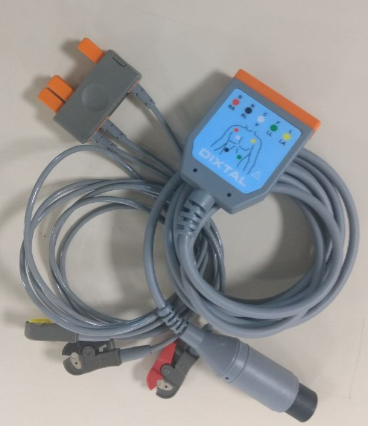
\includegraphics[width=.5\textwidth]{Figuras/Cabopaciente.PNG}
 			\vspace*{\fill} 
            \begin{quote} 
            \centering 
           Fonte: Elaborada pela autora
            \end{quote}
            \vspace*{\fill}
			\label{fig:cabopaciente}
\end{center}
\end{figure}

\subsubsection{Simulador de Sinais Vitais}
\hspace*{0.8cm} No mercado existem diversos modelos de simulador de sinais vitais que simulam ondas no formato analógico. A diferença é que alguns possuem 5 pinos, ou seja é limitado para algumas derivações e outros possuem 10 pinos, que geram todas as derivações. O mais avançado neste ramo é conhecido como PROSIM4- FLUKE, desenvolvido para gerar as 12 formas de derivações ECG e oferece simulações com os parâmetros de marca-passo, teste de arritmia, respiração, pressão invasiva, temperatura, débito cardíaco, simulação de ECG fetal/materno. Por possuir diversas funcionalidades, seu preço é elevado quando comparado a outros equipamentos. Este modelo é demonstrado na Figura \ref{fig:simvitais}.

\begin{figure}[H]
\begin{center}
			\caption{Simulador de sinais vitais - PROSIM3-FLUKE}
			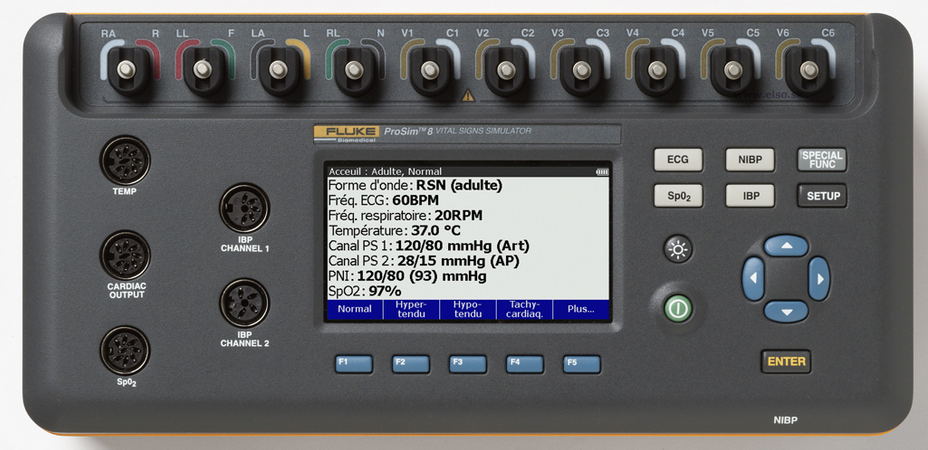
\includegraphics[width=.4\textwidth]{Figuras/fluke.png}
			\vspace*{\fill} 
            \begin{quote} 
            \centering 
           Fonte: \cite{fluke}
            \end{quote}
            \vspace*{\fill}
			\label{fig:simvitais}
\end{center}
\end{figure}

O HS-15 é o modelo utilizado nesse projeto para teste e gerar os sinais vitais em modo ECG. Este simulador permite alterar frequência, amplitude e opera  em cinco modos que fornecem a forma de onda quadrada, triangular, seno, pmp e ECG.  O pulso de ECG pode ser modificado em 30-60-80-120-180-240 btm. 
	

A Figura \ref{fig:hs15} representa o simulador de sinais HS-15 da empresa Handy Sim, desenvolvido para ser utilizado em procedimento de verificação de parâmetro, manuntenção, avaliação de desempenho, teste e calibração em monitores cardíacos e eletrocardiógrafo. 
 

%http://catalogohospitalar.com.br/hs15-simulador-de-ecg-c-12-variacoes-para-eletrocardiografo-multicanal.html

\begin{figure}[H]
\begin{center}
			\caption{Simulador HS-15}
			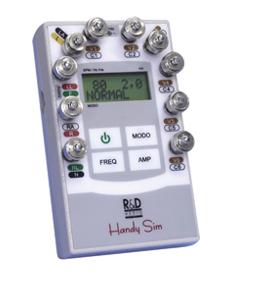
\includegraphics[width=.4\textwidth]{Figuras/HS150.PNG}
			\vspace*{\fill} 
            \begin{quote} 
            \centering 
           Fonte: \cite{HS15}
            \end{quote}
            \vspace*{\fill}
			\label{fig:hs15}
  
\end{center}
\end{figure}

\newpage


\section{IMPLEMENTAÇÃO DO PROJETO}

\hspace*{0.8cm} Este capítulo aborda o desenvolvimento do módulo de aquisição do sinal ECG incluindo o circuito de aquisição de sinal, contemplando a conversão analógico-digital e a transmissão do sinal ECG. O diagrama esquemático deste sistema está exposto na  Figura \ref{fig:dia}. Deste diagrama, tem-se os eletrodos, que estão conectados no paciente; o cir\-cuito de aquisição para tratar e acomodar o sinal enquanto o MCP3008 é utilizando como conversor analógico/digital e se conecta com o Raspberry Pi 3 através da porta SPI. Ambos estão configurados para transmitir o sinal ECG. O sistema é iniciado com o pedido realizado pelo usuário, utilizando a arquitetura cliente-servidor presente nos computadores. Internamente o cliente
faz a requisição ao servidor presente no Raspberry Pi 3 e o interpreta, utilizando a rede Wi-Fi como meio de comunicação, realizando a leitura de dados da porta do MCP3008, a qual está conectada com o circuito de aquisição e por fim, o cliente recebe as amostras, fornecida pelo o servidor. \textcolor{red}{há extra "espaços"...verifique isso....acho que vc poderia quebrar esse para em dois e explicar um pouco melhor}


\begin{figure}[H]
\begin{center}
			\caption{Diagrama Esquemático do Sistema Proposto}
			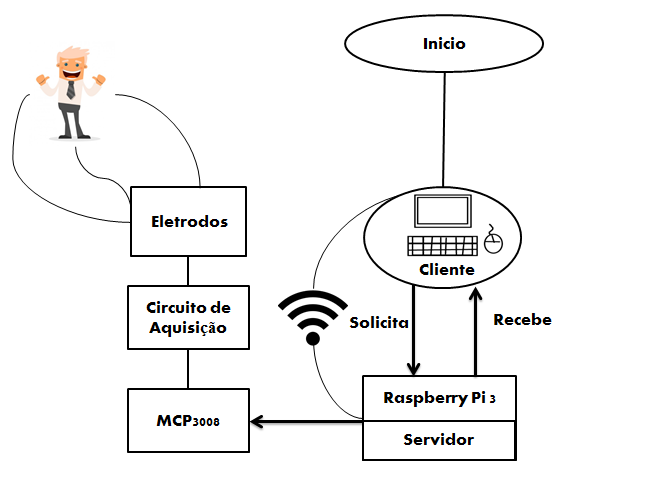
\includegraphics[width=.8\textwidth]{Figuras/diaG.PNG}
            \vspace*{\fill} 
            \begin{quote} 
            \centering 
           Fonte: {Elaborada pela autora}
            \end{quote}
            \vspace*{\fill}
			\label{fig:dia}

\end{center}
\end{figure}



\subsection{DESENVOLVIMENTO DO HARDWARE}
\hspace*{0.8cm}Após a etapa de definição e aquisição de componentes que fazem parte da configuração do hardware, procedeu-se a implementação do circuito eletrônico em um protoboard, sendo que inicialmente foram realizados testes nos componentes eletrônicos. O primeiro teste consistiu na verificação dos sinais ECG utilizando a placa ECG AD8232, a qual foi alimentada com a tensão de 3,3V e utilizou o  pino GND para aterramento do sinal. Utilizou-se os pinos RA, LA e RL do simulador de sinais vitais HS-15 no modo ECG, conectado nos pinos RA, LA e RL da placa AD8232 com o intuito de analisar a forma de onda característica do sinal ECG, com o manuseio da ponta de prova do osciloscópio e assim analisar o sinal na tela do equipamento. \textcolor{red}{verifique os "espaços" novemente}


A segunda parte é realizar e estabelecer a comunicação entre o Raspberry Pi 3 e o MCP3008. Para a leitura de dados fornecedido pelo o conversor analógico-digital, bibliotecas foram instaladas, utilizando os terminais do Raspberry (19, 21, 23, 24 e 26) para que ambos conectasse através da conexão serial SPI que possuem. A conexão foi realizada da seguinte forma: os pinos VDD, VREF, AGND, CLK, DOUT, DIN, CS/SHDN e DGND do MCP3008 foram conectados ao Raspberry Pi de acordo  a pinagem estabalecida na Tabela 3. \textcolor{red}{corrija: fornecido, conectasse....a espaços extras novamente...}

\textcolor{red}{Os testes foram realizados em cada porta, ou seja, inserindo qualquer sinal as porta de entradas CH0, CH1, CH2, CH3, CH4, CH5, CH6, CH7 e os valores gerados no Raspberry em tempo real, qualquer alteração que é feito nas portas de entrada é imediatamente alterado a leitura da porta que esta sendo utilizada}. Os valores das 08 portas de entradas são exibidos em uma tabela contendo os valores de canal e, a cada meio segundo, uma nova linha é impressa com os novos valores do canal. Cada coluna representa um canal específico da porta de entrada no MCP3008 e esses valores variam de 0 a 1023, onde 0 significa que o sinal está no nível do terra (GND) e 1023 significa que ele está no valor VREF (3,3V) ou superior. \textcolor{red}{O TEXTO QUE EU MARQUEI EM VERMELHO DEVERÁ SER ESCRITO DE UM MODO MELHOR...parece que falta virgula e uma preposição}

\begin{table}[H]
\centering
\caption{Conexão dos Pinos}
\begin{center}
\label{my-label}
\begin{tabular}{|c|c|}
\hline
\multicolumn{2}{|c|}{\textbf{Pinos}} \\ \hline
\multicolumn{1}{|l|}{\textbf{MCP3008}} & \multicolumn{1}{l|}{\textbf{Raspberry Pi}} \\ \hline
16 & 01 \\ \hline
15 & 01 \\ \hline
14 & 05 \\ \hline
13 & 23 \\ \hline
12 & 21 \\ \hline
11 & 19 \\ \hline
10 & 24 \\ \hline
9 & 39 \\ \hline
\end{tabular}
\end{center}
 \vspace*{\fill} 
            \begin{quote}
            \centering 
            \vspace{12pt}Fonte: {Elaborada pela autora} 
            \end{quote}
            \vspace*{\fill}
			\label{fig:ramcor}
\end{table}


A Figura \ref{fig:lop} representa a primeira disposição de componentes no protoboard que foi desenvolvido através de uma plataforma de software aberta chamada Fritzing \textcolor{red}{aqui vai uma ref} , na qual é possivel ao usuário documentar protótipo, esquematizar placa, layout de placa, entre outras funções. 
\begin{figure}[H]
\begin{center}
			\caption{Circuito Esquemático}
			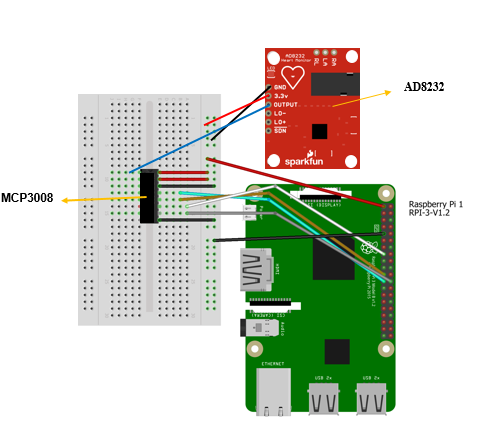
\includegraphics[width=.6\textwidth]{Figuras/PROT.PNG}
			 \vspace*{\fill} 
            \begin{quote} 
            \centering 
           Fonte: {Elaborada pela autora}
            \end{quote}
            \vspace*{\fill}
			\label{fig:lop}
\end{center}
\end{figure}
O circuito esquemático desenvolvido contém os seguintes componentes: placa front-end \textcolor{red}{explique o que é isso}, MCP3008 e Raspeberry. A confecção da parte inferior da placa está demonstrada especificamente na Figura \ref{fig:esque}. Nota-se que a placa possui dois segmentos traçados que são jumper soldado na parte superior da placa universal.
\begin{figure}[H]
\begin{center}
			\caption{Representação inferior da trilha da placa universal}
			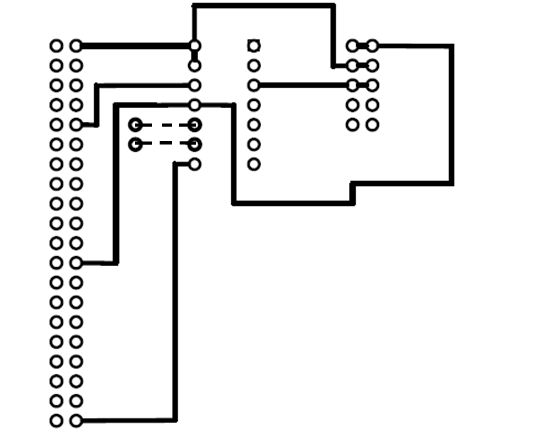
\includegraphics[width=.5\textwidth]{Figuras/ofic.png}
               \vspace*{\fill} 
            \begin{quote} 
            \centering 
           Fonte: Elaborada pela autora

            \end{quote}
            \vspace*{\fill}
			\label{fig:esque}
\end{center}
\end{figure}

Na prática esse circuito esquemátizado é montado no protoboard, conforme a Figura \ref{fig:esquem}, porém nessa imagem o conversor e o raspberry já estão configurados para amostragem do sinal ECG. Destaca-se o excesso e a desordem de jumper conectados nos componentes e protoboard. Os sinais obtidos do simulador são amplificados e tratados através da placa fornecida pela  Sparkfun. Os dados são lidos na porta e convertido em sinais digitais e transferidos para o Raspberry através do protocolo SPI. \textcolor{red}{vc escreveu "esquematizado" de maneira errada}

Para a amplificação dos sinais característico a onda de ECG os pinos da Placa Front-End RA, LA e RL foram conectados especificamente em cada pino RA, LA e RL do simulador de sinais vitais no modo ECG. A conexão entre o HS-15 e a Placa Front-End é feita através de cabos. Esses cabos são de grande importância, pois isolam o paciente do circuito externo. Utilizou-se o produto cabo paciente ecg 5 vias da empresa Dixtal Philips, o qual foi modificado para o circuito, pois fornece apenas três vias RA, LA, RL e com isso retirou-se as vias V e LL. \textcolor{red}{há erro de concordância em característico}

Após a realização da montagem dos componentes no protoboard, observou-se a necessidade de eliminar jumper, pois causava interferência no circuito. Assim, foi confeccionada uma placa de fabricação manual com apenas  conectores: o primeiro conector tipo macho de 20 pinos para inserir o cabo flat do raspberry, conector fêmea para inserir o próprio MCP3008, 2 conectores para a placa front-end um conector fêmea para os pinos GND, 3,3V e OUTPUT e outro macho para conectar com os pinos RA, LA e RL com o conector do cabo paciente.

\begin{figure}[H]
\begin{center}
			\caption{Representação inferior da trilha da placa universal}
			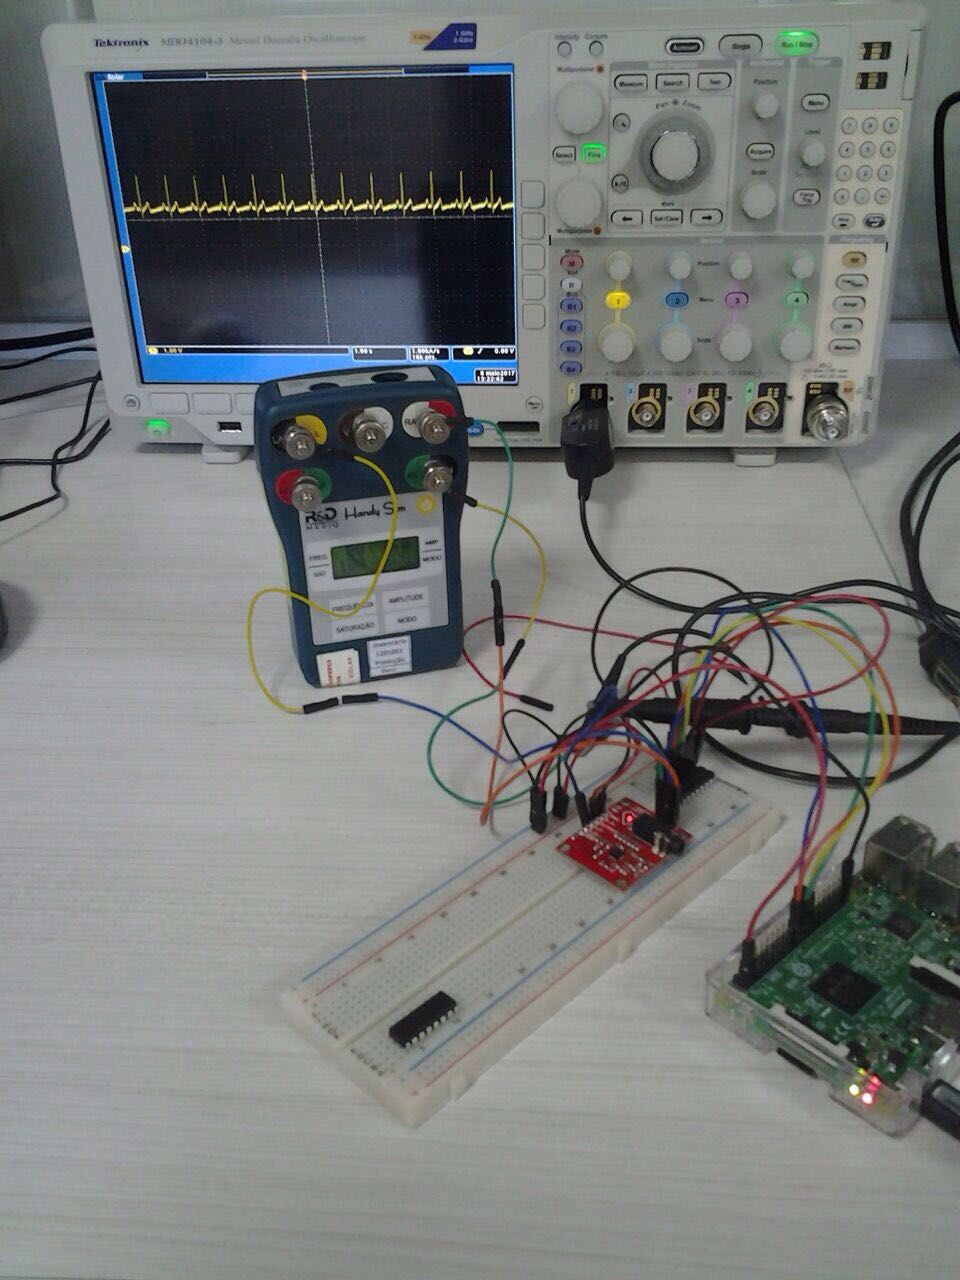
\includegraphics[width=.5\textwidth]{Figuras/pop.jpeg}
             \vspace*{\fill} 
            \begin{quote} 
            \centering 
           Fonte: Elaborada pela autora
            \end{quote}
            \vspace*{\fill}
			\label{fig:esquem}
\end{center}
\end{figure}

Com base na representação inferior da trilha da placa inferior foi possível desenvolver a mesma representação na placa de circuito confeccionada para o projeto, para isso utilizou-se apenas solda de estanho-chumbo  e estação de solda. A Figura \ref{fig:trilhainfesup} exibe a parte inferior e superior da placa confeccionada. Na esquerda tem-se a representação inferior enquanto na direita tem-se a parte superior. \textcolor{red}{erro: espaços extras}


A região inferior tem-se apenas pinos de conexão e solda estanho-chumbo e a superior tem-se apenas os conectores para inserir os componentes para conexão da placa, conversores e Raspeberry. A placa confeccionada foi inserido em uma caixa para proteger o circuito.

\begin{figure}[H]
\begin{center}
			\caption{Representação inferior da trilha da placa universal}
			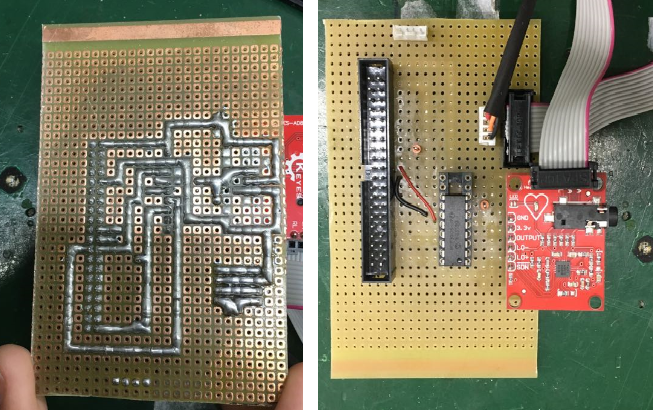
\includegraphics[width=.9\textwidth]{Figuras/pl.PNG}
             \vspace*{\fill} 
            \begin{quote} 
            \centering 
         Fonte: Elaborada pela autora
            \end{quote}
            \vspace*{\fill}
			\label{fig:trilhainfesup}
\end{center}
\end{figure}

\subsection{FIRMWARE}
\hspace*{0.8cm}O Raspberry foi programado para ler os dados fornecido pelo o MCP3008 durante a utilização do simulador conectado a placa amplificadora. Para tal finalidade é necessário fazer uso de bibliotecas que precisam esta \textcolor{red}{<-ESSA PALAVRA ESTÁ ERRADA} instalada no terminal do Raspberry. Após a conexão  da fiação ser conectada, instalar a biblioteca Adafruit MCP3008 Python fornecido pela a plataforma aberta GitHub \textcolor{red}{AQUI VAI UMA REF}. A partir da fonte do GitHub é necessário que o Raspberry esteja conectado a rede e acessar o terminal com os seguintes comandos nessa ordem especifico \textcolor{red}{<- AJEITE ESSA FRASE} :
\begin{figure}[H]
\begin{center}
		
			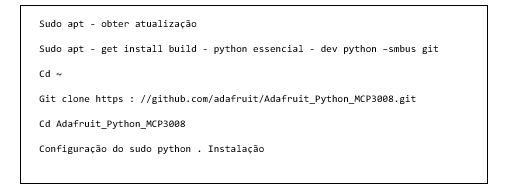
\includegraphics[width=.8\textwidth]{Figuras/com.PNG}
			
\end{center}
\end{figure}

Ao baixar as bibliotecas através da plataforma é necessário modificar a pasta de acesso para Adafruit/Python/MCP3008, nesse repositorio é necessário modificar simpleteste.py e alterar a configuração do Software de acordo com a pinagem entre o conversor e o raspberry estabelecida:
\begin{itemize}
\item MCP3008 VDD para Raspberry Pi 3,3V
\item MCP3008 VREF paraa Raspberry Pi 3,3V
\item MCP3008 AGND para Raspberry Pi GND
\item MCP3008 DGND para Raspberry Pi GND
\item MCP3008 CLK para Raspberry Pi SCLK
\item MCP3008 DOUT para Raspberry Pi MISO 
\item MCP3008 DIN para Raspberry Pi MOSI
\item MCP3008 CS/SHDN Raspberry Pi CE0
\end{itemize}

Ao executar o comando na porta do raspberry, o programa imprimirá uma tabela com todos os canais ADC e seus valores. A cada meio segundo, uma nova linha será impressa com os mais recentes valores de canal.

Cada coluna representa um canal diferente e o cabeçalho da primeira linha mostra o número do canal (de 0 a 7, 8 canais no total). O valor para cada canal é o valor ADC para esse canal. Este é um número que varia de 0 a 1023, onde 0 significa que o sinal está no nível do solo e 1023 significa que ele está no valor VREF (3,3V) ou superior. Os outros valores são obtidos por relação proporcional, por exemplo, um valor de 512 é 3,3 / 2 ou 1,65 volts. \textcolor{red}{NIVEL DO SOLO????? NÃO DÁ PARA UTILIZAR OUTRO TERMO???}

O MCP3008 possui 8 portas de leitura de sinais, para a configuração do projeto usou-se a porta 04 para a leitura da placa de aquisição, essa leitura é mostrada na Figura \ref{fig:ciru}. Para configuração cliente-servidor foi utilizado a estrutura web Pyhton Tornado versão 4.5.2 fornecido pela fonte github. O tornado pode ser utilizado para conexões abertas, pesquisas longas, WebSocket ou aplicações que exigem uma conexão longa para o usuário. Neste caso é utilizado o protocolo de comunicação HTTP-(\textit{HyperText Transfer Protocol}) \textcolor{red}{AQUI VAI UMA REF}, o qual permite a estrutura de cliente-servidor, proposta neste trabalho. Uma requisição é caracterizada por uma mensagem HTTP enviada de um cliente para um servidor e a resposta é caracterizada por uma mensagem HTTP enviada por um servidor a um cliente.

A comunicação é feita através da porta 8888. Utilizou-se os códigos em Phython do cliente e servidor, fornecido no APÊNDICE A, utilizando como meio de comunicação o protocolo definido. Para isto configurou a rede Wi-Fi para o meio de comunicação. \textcolor{red}{VC ESCREVEU ERRADO "CONFIGUROU"...LEIA NOVAMENTE A FRASE}  

\begin{figure}[H]
\begin{center}
			\caption{Leitura da porta do MCP3008}
			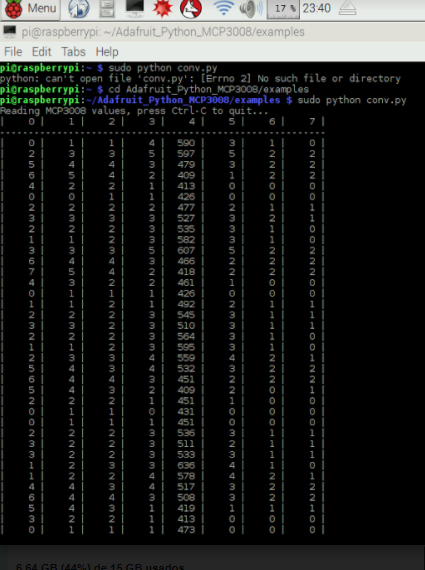
\includegraphics[width=0.6\textwidth]{Figuras/D.PNG}
              \vspace*{\fill} 
            \begin{quote} 
            \centering 
           Fonte: Elaborada pela autora
            \end{quote}
            \vspace*{\fill}
			\label{fig:ciru}
\end{center}
\end{figure}
Para o uso das sintaxes do código cliente e servidor, é necessário utilizar a fonte do github e importar algumas bibliotecas para manipulação de dados. Foram importados as bibliotecas contidos na código cliente e servidor para a utilização do código.

O cliente faz requisição e o servidor o responde na ordem da solicitação. A função urllib2 presente no código cliente  é uma função do Python usado para obter URLs. Nesse caso a busca é realizada usando protocolo 
HTTP, o qual é baseado em solicitar e responder. O acesso é feito pelo o endereço do IP do servidor acessando a porta 8888 do Raspberry pi 3. \textcolor{red}{ESPAÇOS NOVAMENTE KKKKK}

O diagrama da Figura \ref{fig:kenny}, baseia-se na seguinte proposta: o cliente faz requisição ao servidor o qual acessa a porta 8888 do Raspberry. Nesta porta está sendo executado o Tornado, o qual manipula a solicitação HTTP. O servidor comunica-se através do protocolo SPI com o conversão MCP3008 e faz a leitura de 10000 pontos da porta 4 do MCP3008 fornecido pelo o sistema de aquisição. Esses dados são transmitidos ao cliente em forma de lista e o mesmo manipula para a geração do gráfico.

 
 \begin{figure}[H]
\begin{center}
			\caption{Diagrama do projeto Cliente-Servidor}
			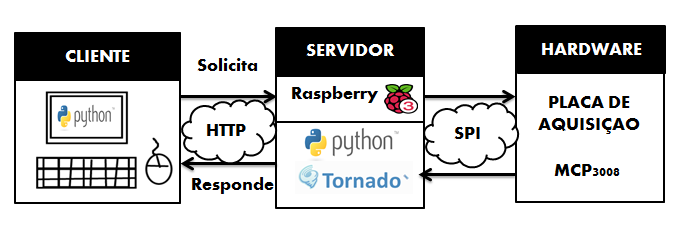
\includegraphics[width=1\textwidth]{blocos.PNG}
              \vspace*{\fill} 
            \begin{quote} 
            \centering 
           Fonte: {Elaborada pela autora} 
            \end{quote}
            \vspace*{\fill}
			\label{fig:lopioupe}
            \vspace*{\fill}
			\label{fig:kenny}
\end{center}
\end{figure}
 
\newpage

\section{RESULTADOS}

\hspace*{0.8cm} Neste capítulo são abordados os resultados obtidos durante o desenvolvimento do trabalho de conclusão de curso. Destaca-se neste projeto dois resultados significativos, um deles é o protótipo físico desenvolvido, apresentado na Figura \ref{fig:mama} e o outro resultado diz respeito as formas de ondas obtidas que compõe mo sinal de ECG, formando pela onda P, complexo QRS e onda T. \textcolor{red}{E O BAIXO CUSTO????}

Os componentes utilizados na montagem do protótipo são apresentados no capítulo 3. Após, as etapas de montagem, soldagem e configuração, realizou o acomodamento do sistema, para isso utilizou uma caixa patola deixando apenas um espaço destinado conexão do cabo-flat com os pinos do Raspberry e a entrada do cabo paiciente, destaca-se que esse tipo de caixa é amplamente utilizada para acabamento estético, proteção de circuitos. A Figura \ref{fig:mama}, representa o dispositivo final, disposto na caixa patola.




\begin{figure}[H]
\begin{center}
			\caption{Dispositivo final, disposto na caixa patola}
			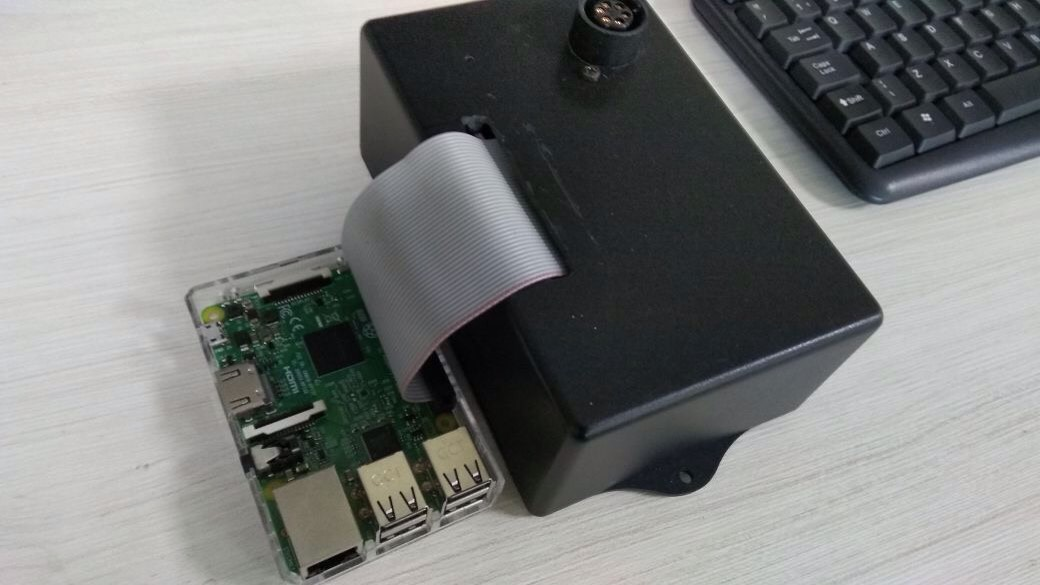
\includegraphics[width=.9\textwidth]{Figuras/IMG_3651.jpg}
              \vspace*{\fill} 
            \begin{quote} 
            \centering 
           Fonte: Elaborada pela autora
            \end{quote}
            \vspace*{\fill}
			
			\label{fig:mama}
\end{center}
\end{figure}
A utilização da placa baseada no CI AD8232 da Analog Device para obtenção dos sinais de ECG foi importante para eliminar as variáveis do processo de aquisição. O protótipo desenvolvido foi testado com o simulador de sinais vitais HS-15, e seus resultados foram comparados aos resultados da forma de onda padrão da segunda derivação eletrocardiográfica de um equipamento comercial modelo EP-12 da empresa Philips Dixtal \textcolor{red}{AQUI VAI UMA REF}.

A Figura \ref{fig:popi}, representa o sinal ECG simulado no equipamento eletrocardiógrafo EP12, o equipamente utiliza o mesmo modelo de simulador de sinais vitais utilizando neste trabalho. É possivel, analisar e verificar a semelhança com a o sinal exposto na Figura  \ref{fig:oscilo}.  O propósito deste projeto é fornecer com qualidade e parâmetros as formas de ondas característica do ECG. \textcolor{red}{MELHORE ESSA ULTIMA FRASE}

\begin{figure}[H]
\begin{center}
			\caption{Sinal de ECG simulado no EP12 Dixtal}
			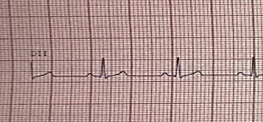
\includegraphics[width=.8\textwidth]{Figuras/exame.PNG}
              \vspace*{\fill} 
            \begin{quote} 
            \centering 
           Fonte: \cite{ronald}
            \end{quote}
            \vspace*{\fill}
			\label{fig:popi}
\end{center}
\end{figure}

A Figura \ref{fig:oscilo}, representa a forma de onda adquirida pelo o sistema de aquisição, utilizando o simulador para gerar sinais vitais e o oscilóscopio para análise. Este sinal é composto pela a onda p, complexo QRS e a onda T, característico da forma de onda do eletrocardiograma. \textcolor{red}{MELHORE ESSE PARA...ESCREVA MAIS OU MENOS ASSIM: NA FIGURA TAL, APRESENTA-SE A FORMA DE ONDA....SACOU??...EM GERAL, PROCURE ESCREVER ASSIM...OU SEJA, CORRIJA O RESTO...}

\begin{figure}[H]
\begin{center}
			\caption{Sinal do ECG obtido pelo o osciloscópio}
			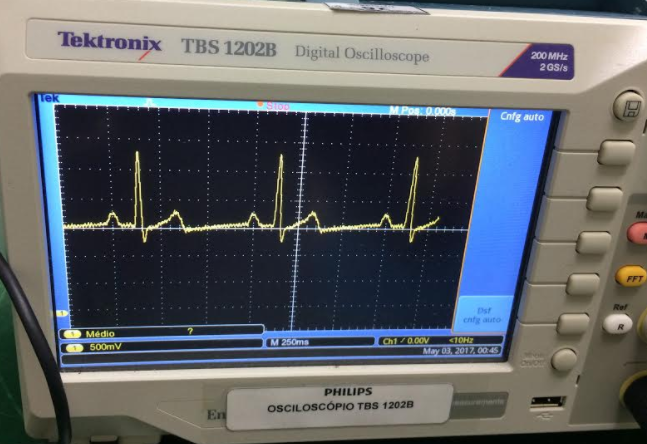
\includegraphics[width=.9\textwidth]{Figuras/oscil.PNG}
             \vspace*{\fill} 
            \begin{quote} 
            \centering 
           Fonte: Elaborada pela autora
            \end{quote}
            \vspace*{\fill}
			\label{fig:oscilo}
\end{center}
\end{figure}

\hspace*{0.8cm}O Raspberry Pi 3 está sendo usado como servidor. O cliente solicita através do comando 'req' e para cada amostra é determinado um valor de acordo com o sinal fornecido pelo o simulador através da porta do mcp.read-adc(4), ou seja, a porta 4 do conversão analogico/digital. Essa leitura está sendo comprovado na Figura \ref{fig:kiki}.

\begin{figure}[H]
\begin{center}
			\caption{Amostragem Sinal do ECG}
			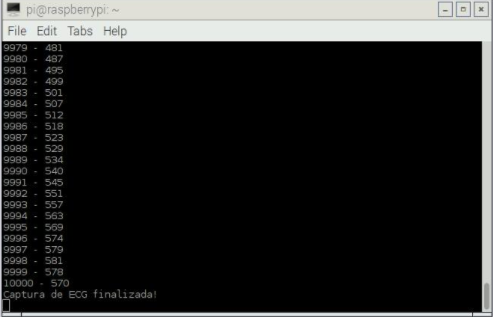
\includegraphics[width=.9\textwidth]{Figuras/json.PNG}
			              						\vspace*{\fill} 
            \begin{quote} 
            \centering 
           Fonte: Elaborada pela autora
            \end{quote}
            \vspace*{\fill}
			\label{fig:kiki}
\end{center}
\end{figure}

Os testes de transmissão e recepção do sinal utilizando a arquitetura cliente-servidor proposta foram realizados conectando os dispositivos através da rede Wi-fi do HUB. Com o resultado dessa arquitetura, tem-se a forma de onda utilizando o simulador de sinais vitais, conectado ao protótipo. Nestes testes, utilizou-se o simulador e foi variado a amplitude e o batimento por minuto.

A Figura \ref{fig:ecg2}, representa um resultado da arquitetura e o protótipo. A imagem representa o sinal ECG simulado, composto por 500 amostras de amplitude do sinal em determinado tempo. Esse sinal é composto inicialmente pela a onda P, complexo QRS e seguindo a onda T. 


\begin{figure}[H]
\begin{center}
			\caption{Sinal ECG simulado}
			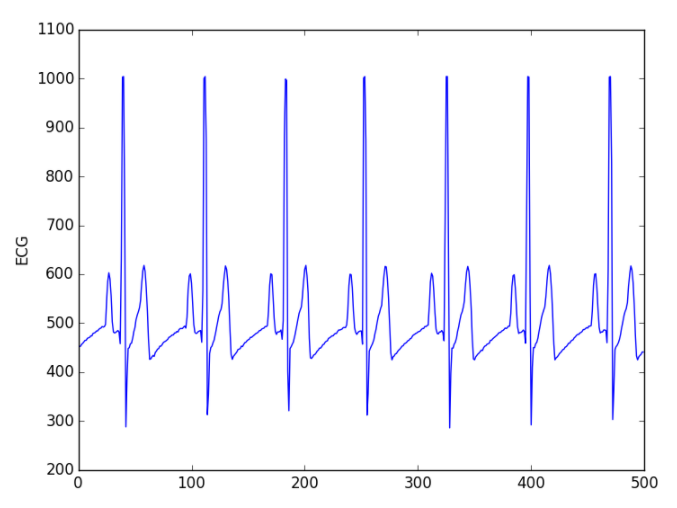
\includegraphics[width=.8\textwidth]{Figuras/sinal.PNG}
                          						\vspace*{\fill} 
            \begin{quote} 
            \centering 
           Fonte: Elaborada pela autora
            \end{quote}
            \vspace*{\fill}
			\label{fig:ecg2}
\end{center}
\end{figure}
\begin{figure}[H]

\hspace*{0.8cm}Para a validação do sistema proposto, o usuário solicita através de comando utilizando o cliente, o qual requisita ao servidor usando topologia estabelicida, o qual faz a leitura de dados e a transfere para o servidor. A Figura \ref{fig:syst}, exibe o sistema em operação: uma tela está exibindo a resposta solicitada ao servidor, ou seja, o sinal ECG adquirido pelo sistema de aquisição utilizando sinais fornecido pelo o  simulador de sinais vitais e a outra tela, apenas faz a exibição da leitura do MCP3008.

\begin{center}
			\caption{Sistema em Operação}
			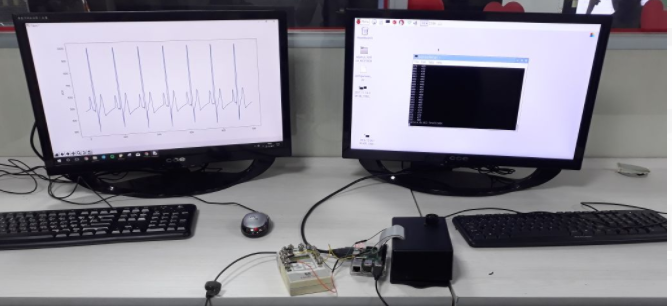
\includegraphics[width=.9\textwidth]{sist.PNG}
            	\vspace*{\fill} 
            \begin{quote} 
            \centering 
           Fonte: Elaborada pela autora
            \end{quote}
            \vspace*{\fill}
			\label{fig:syst}
\end{center}
\end{figure}

\newpage
\vspace*{4cm}
\begin{center}
\textbf{CONCLUSÃO}
\end{center}
\vspace{48pt}

\textcolor{red}{FALTOU FALAR DO BAIXO CUSTO...OU RETIRAMOS ESSA CONTRIBUIÇÃO...}


\addcontentsline{toc}{section}{CONCLUSÃO}

\hspace*{0.8cm}O objetivo deste trabalho foi desenvolver um  protótipo de aquisição de sinais eletrocardiográficos portátil de baixo custo, para obter as ondas P, complexos QRS e ondas T. Inicialmente, realizou-se uma revisão das áreas de conhecimento relativo aos sinais que constituem o eletrocardiograma, estrutura de aquisição e transmissão de dados, tendo em vista atender a proposição do trabalho de pesquisa.

O protótipo desenvolvido, conseguiu atender as especificações iniciais, gerando resultados satisfatórios que permitem a análise do sinal e a comunicação com um computador em tempo real, através apenas de uma solicitação utilizando uma rede de acesso sem fio, empregando o protocolo 802.11.

Com base no protótipo desenvolvido, é possível analisar diretamente a forma de onda P, complexo QRS e onda T, e verificar a influência do batimento cardíaco sobre o sinal. Foram realizados testes com a frequência mínima de 30 btm e frequência máxima de 240 btm, para assim,  determinar a oxigenação do corpo e possíveis disfunções à saúde, ou até mesmo casos críticos que podem levar a morte repentina. \textcolor{red}{ESPAÇOS NOVAMENTE}

Ao decorrer do trabalho surgiram novas implementações que  foram desenvolvidas, porém sem êxito, sendo uma destas a implementação do cabo paciente. O protótipo foi desenvolvido para receber a conexão do cabo paciente (AE-0H002-0) , porém os resultados da forma de onda ECG, não foram satisfatórios \textcolor{red}{TU MOSTROU ISSO NO CAP DE RESULTADOS??? SE NÃO, COLOQUE}. Outras ideias para melhoria do sistema não foram desenvolvidas, devido ao espaço de tempo limitado e a complexidade envolvida \textcolor{red}{<- TIRE ESSA FRASE}. Este trabalho permite diversas novas aplicações, e deixa em aberto possibilidades para melhorias e  desenvolvimento de outros trabalhos correlatos.

Com base nisso merecem destaque os seguintes trabalhos futuros.

\begin{itemize}
\item Eliminar os ruídos presente na forma de onda que compõe o ECG.
\item Melhoria do cabo paciente (AE-0H002-0).
\item Criação de uma interface gráfica que atendam as necessidade do usuário.
\end{itemize}

Independentemente destas etapas não terem sido incorporadas no protótipo, o mesmo já foi projetado visando incorporar estas futuras melhorias, permitindo a continuidade do projeto.

\newpage


% Uncomment the following two lines if you want to have a bibliography. Please do not forget to add an entry to your bibliography and reference it by using the \cite{} command
%\bibliographystyle{alphadin}
\providecommand*{\refname}{}
\renewcommand*{\refname}{\begin{center}\textbf{REFERÊNCIAS}\end{center}}

\newpage
\vspace*{4cm}
%\providecommand{\bibname}{}
%\renewcommand{\bibname}{\begin{center}\textbf{REFERÊNCIAS}\vspace{48pt}\end{center}}

\pagestyle{empty}
\pagestyle{myheadings}

%\bibliographystyle{alpha}

\addcontentsline{toc}{section}{REFER\^ENCIAS}
\bibliography{bibliografia}

\newpage
%\pagestyle{fancy}
%\renewcommand{\headrulewidth}{0pt}
%\rhead{\thepage}
%\fancyfoot[C]{}
\begin{center}
\textbf{APÊNDICE A-  CLIENTE/SERVIDOR}

\addcontentsline{toc}{section}{APÊNDICE A - CLIENTE/SERVIDOR}


\textbf{CLIENTE}

\lstinputlisting[language={Python},inputencoding={utf8},extendedchars=false]{cliente.py}


\newpage
\textbf{SERVIDOR}

\lstinputlisting[language={Python},inputencoding={utf8},extendedchars=false]{servidor.py}

\end{center}

\newpage
\begin{center}
\textbf{APÊNDICE B - SINAIS ECG OBTIDOS PELO O SISTEMA DE AQUISIÇÃO}

\addcontentsline{toc}{section}{APÊNDICE B - SINAIS ECG OBTIDOS PELO O SISTEMA DE\newline AQUISIÇÃO}
\begin{itemize}
\item Amplitude 0,5mV
\begin{figure}[H]
\begin{center}
\caption{Sinal ECG 30 bpm}
					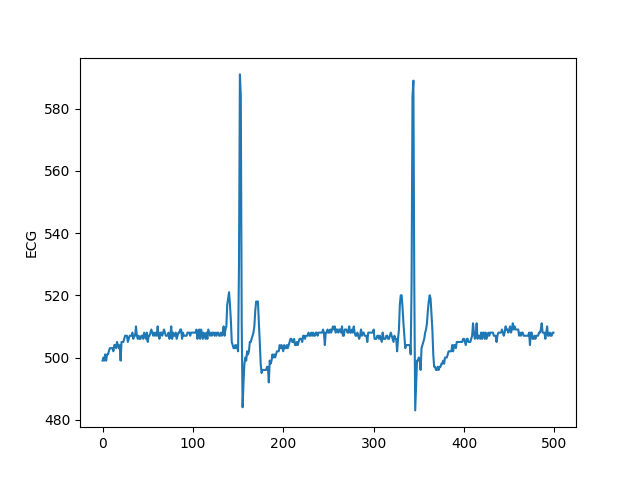
\includegraphics[width=0.7\textwidth]{Figure_1-1.png}
			     \vspace*{\fill} 
            \begin{quote} 
            \centering 
            Fonte: (Acervo da Autora, 2017)
            \end{quote}
            \vspace*{\fill}
			\label{fig:eletrodo}
\end{center}
\end{figure}



\newpage

\item Amplitude 1,5mV

\begin{figure}[H]
\begin{center}
\caption{Sinal ECG 30 bpm}
		
			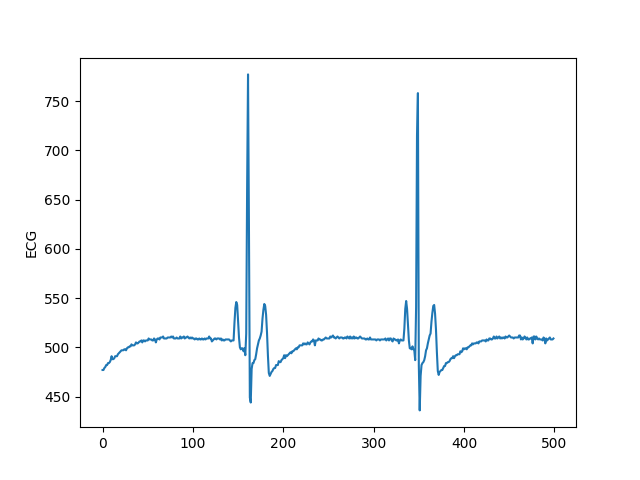
\includegraphics[width=0.7\textwidth]{Figure_3-1.png}
       \vspace*{\fill} 
            \begin{quote} 
            \centering 
            Fonte: Elaborada pela autora
            \end{quote}
            \vspace*{\fill}
			\label{fig:eletrodo}
\end{center}
\end{figure}

\end{itemize}

\end{center}

% End of the document
\end{document}
